\documentclass[12pt,a4paper,oneside]{erdc}
%\documentclass{erdc}
\usepackage[T1]{fontenc}		% Selecao de codigos de fonte.
\usepackage[utf8]{inputenc}		% Codificacao do documento (conversão automática dos acentos)
%\usepackage{lastpage}			% Usado pela Ficha catalográfica
\usepackage{indentfirst}		% Indenta o primeiro parágrafo de cada seção.
\usepackage{color}				% Controle das cores
\usepackage{graphicx}			% Inclusão de gráficos
%\usepackage{microtype} 			% para melhorias de justificação
\usepackage[brazil]{babel}
%\usepackage[brazilian,hyperpageref]{backref}	 % Paginas com as citações na bibl
%\usepackage[alf]{abntex2cite}	% Citações padrão ABNT
\usepackage{hyperref}
\usepackage{natbib}

\usepackage{lipsum}


\usepackage{Sweave}
\begin{document}
\Sconcordance{concordance:BP_Curso_TecComp_00_2019.tex:/home/rivero/Dropbox/Workspace_Current/Projects/EmExec/Banpara/Cursos/git_curso/curso_intro_datascience/Apostilas/BP_Curso_TecComp_00_2019.Rnw:%
1 18 1 1 0 92 1 1 5 352 1}
\Sconcordance{concordance:BP_Curso_TecComp_00_2019.tex:/home/rivero/Dropbox/Workspace_Current/Projects/EmExec/Banpara/Cursos/git_curso/curso_intro_datascience/Apostilas/BP_Curso_TecComp_00_c08_2019.Rnw:ofs 465:%
1 13 1}
\Sconcordance{concordance:BP_Curso_TecComp_00_2019.tex:/home/rivero/Dropbox/Workspace_Current/Projects/EmExec/Banpara/Cursos/git_curso/curso_intro_datascience/Apostilas/BP_Curso_TecComp_00_2019.Rnw:ofs 479:%
470 28 1}


\frontmatter

\laboratory{PPGE-UFPA}

\reportnum{BP/EcoS - Curso-DataScience-00-2019}

\program{Construção de Modelos e Indicadores Econômicos}

\title{Introdução ao Tratamento \\ e Análise de Dados em R}


%\subtitle{ou Data Science para todos!}

\date{\today}

\author{Sérgio Rivero \and Hilder Farias}

\affiliation{Programa de Pós-Graduação em Economia\\
	Instituto de Ciências Sociais Aplicadas\\
	Universidade Federal do Pará\\
	Rua Augusto Correia, 1\\
	Belém, Pará - 66.075-200}

\author{Murilo Gomes, Lais Conte  \and Erwin Braga }


\affiliation{Faculdade de Economia \\
	Instituto de Ciências Sociais Aplicadas\\
	Universidade Federal do Pará\\
	Rua Augusto Correia, 1\\
	Belém, Pará - 66.075-200}


\coverart[width=\linewidth]{../figs/Capa}

\reporttype{Produto: Cursos}

\distribution{Propriedade BANPARÁ e PPGE-UFPA \\ (Distribuição Restrita)}

% \distribution{Distribution authorized to U.S. Government Agencies
% only; Test and Evaluation; November 2005.  Other requests should be
% referred to U.S. Army Engineer Research and Development Center}

%\additionalinfo{Supersedes ERDC/CREL AF-01-23}

%\begin{abstract}
%  \lipsum[12-13]
%\end{abstract}

\disclaimer{
	
	This document is an output from the  Banpará Project 
	
	PPGE-UFPA report
	
	Distribution Restrictions
	
	\copyright 2019, All rights reserved
	
	\pagebreak
	
	}

\preparedfor{Banpará} 

\contractnum{FADESP-NO-CONTRATO}

\monitoredby{Banpará}

%\preparedfor{}




\maketitle

\tableofcontents


%\chapter*{Resumo Executivo}


\mainmatter

%%%%%%%%%%%%%%%%%%%%%%%%%%%%%%%%%%%%%%%%%%%%%%%%%
%  Chamadas de Bibliotecas e Variaveis Globais
%%%%%%%%%%%%%%%%%%%%%%%%%%%%%%%%%%%%%%%%%%%%%%%%%




%%%%%%%%%%%%%%%%%%%%%%%%%%%%%%%%%%%%%%%%%%%%%%%%%%%%%%%%%
%
%    CAPITULO
%
%%%%%%%%%%%%%%%%%%%%%%%%%%%%%%%%%%%%%%%%%%%%%%%%%%%%%%%%%
%
% !Rnw root = BP_Curso_TecComp_00_2019.Rnw


\chapter{Introdução}

O R é uma suíte integrada de software que permite a recuperação, o tratamento, e a análise de dados\cite{Venables2011}. Pode se dizer que o R é um ambiente de tratamento de dados que permite ao usuário, além a análise de dados propriamente dita, escrever extensões e ampliar o seu escopo.

R é uma ferramenta de software livre que atende aos critérios da \textit{Free Software Foundation} e tem uma licença \textbf{GNU}\footnote{\url{https://www.gnu.org/}}

Algumas das funcionalidade do R são\cite{Venables2011}:
\begin{itemize}
	\item Ferramentas para manuseio e armazenamento de dados
	\item Um conjunto de operadores que permitem o cálculo numérico e a manipulação de matrizes
	\item Um enorme conjunto de bibliotecas para análise de dados
	\item Ferramentas para apresentação gráfica de dados e resultados
	\item Uma linguagem de programação orientada a objetos e extensível
	\item A possibilidade de estender a linguagem, suas bibliotecas e funções
\end{itemize}

\begin{figure}
	\centering
	\includegraphics[width=\linewidth]{../figs/f-Intro-01-Monetary-Policy}
	\caption{Exemplo de \textit{Dashboard} de Política monetária usando R \cite{Showmeshiny2019}}
	\label{fig:f-intro-01}
\end{figure}

O R tem um conjunto extenso de ferramentas que permitem desde uma análise simples de regressão ou de aglomerados (\textit{cluster}) até apresentações de resultados extraídos de bancos de dados em larga escala com ferramentas de busca \textit{SQL}\footnote{Structured Query Language - \url{https://pt.wikipedia.org/wiki/SQL}} apresentadas em páginas web (Figura \ref{fig:f-intro-01}).

Neste texto, iremos apresentar um conjunto de ferramentas de uso livre, a sua maioria de código aberto, que permitirão a extração, tratamento, análise e apresentação de dados, tanto para análises estatísticas mais diretas quanto para a tomada de decisões estratégicas de negócios.




%%%%%%%%%%%%%%%%%%%%%%%%%%%%%%%%%%%%%%%%%%%%%%%%%%%%%%%%%
%
%    CAPITULO
%
%%%%%%%%%%%%%%%%%%%%%%%%%%%%%%%%%%%%%%%%%%%%%%%%%%%%%%%%%
%
% !Rnw root = BP_Curso_TecComp_00_2019.Rnw


\chapter{Instalando e Configurando o R e RStudio}


Nesta aula os alunos aprenderão a baixar o R e RStudio bem como aprenderão a utilizar bibliotecas em R


\section{Instalando o R e RStudio}

\subsection{Instalando o R}

Para instalar o R é preciso acessar o site \url{https://www.r-project.org/}. Os passos estão enumerados a seguir:

Nesta página clicar em \textbf{download R} que acessa a página - \url{https://cran.r-project.org/mirrors.html} - (Figura \ref{fig:f01-01})





\begin{figure}[htpb]
	\centering
	\includegraphics[width=\linewidth]{../figs/BP_Curso_TecComp_00_2019_f01-01}
	\caption{Nesta página clicar em \textbf{download R}}
	\label{fig:f01-01}
\end{figure}

Nesta página você seleciona o espelho que utilizará para baixar o R. Há sites no Brasil ou sítios em nuvem o item 0 - Cloud redirecionará automaticamente para sítios apoiados pelo Rstudio  -  \url{https://cloud.r-project.org/} (Figura \ref{fig:f01-02}) - A diferença entre os prefixos \textit{http} e \textit{https} é que os sites com \textbf{"s"} utilizam encriptação. Muitas vezes é necessário utilizar o \textit{https} em instalações cujos ambientes de TI exigem.



\begin{figure}[htpb]
	\centering
	\includegraphics[width=\linewidth]{../figs/BP_Curso_TecComp_00_2019_f01-02}
	\caption{Aqui você seleciona o espelho que vai usar para baixar o R}
	\label{fig:f01-02}
\end{figure}

Você poderá baixar o R (por exemplo em \url{https://cloud.r-project.org/}) ou em algum dos outros espelhos citados anteriormente, de acordo com seu sistema operacional (Figura \ref{fig:f01-03}) Cada sistema (\textit{Linux}, \textit{MacOSX} ou \textit{Windows} tem uma rotina diferente para instalação. Aqui vamos explicar o sistema operacional mais comum (\textit{Windows}). Para outros sistemas, recomenda-se buscar instruções específicas em fóruns adequados.


\begin{figure}[htpb]
	\centering
	\includegraphics[width=\linewidth]{../figs/BP_Curso_TecComp_00_2019_f01-03}
	\caption{Sítio para baixar o R de acordo com seu sistema operacional}
	\label{fig:f01-03}
\end{figure}


Finalmente, para instalar o R, você pode executar o arquivo que está no link apresentado na Figura \ref{fig:f01-04}. Você baixará um arquivo \textbf{.exe} e, ao executá-lo, o instalador do \textit{Windows} tornará o programa disponível para uso na sua máquina. 

\begin{figure}[htpb]
	\centering
	\includegraphics[width=\linewidth]{../figs/BP_Curso_TecComp_00_2019_f01-04}
	\caption{Página do Download do R}
	\label{fig:f01-04}
\end{figure}


Você pode conseguir mais informações sobre o R e os detalhes da instalação checando nos \textit{FAQs}\footnote{Frequently Asked Questions} dos sítios que você estiver acessando \url{https://cloud.r-project.org/bin/windows/base/rw-FAQ.html}, ou em \url{https://cran.r-project.org/doc/manuals/R-admin.html}



\subsection{Instalando o RStudio}

O RStudio é um ambiente de desenvolvimento integrado para o R. Incorpora um conjunto de funções que facilita o desenvolvimento de programas em R e a sua execução. O RStudio não é uma interface gráfica para a execução de rotinas do R, é um ambiente que permite implementar e executar programas. É um pacote comercial com partes de uso livre onde é necessário pagar pelos recursos extras.

\begin{figure}[htpb]
	\centering
	\includegraphics[width=\linewidth]{../figs/BP_Curso_TecComp_00_2019_f01-05}
	\caption{Página inicial do Rstudio}
	\label{fig:f01-05}
\end{figure}

Para iniciar o download da plataforma Rstudio é preciso acessar o site (\url{https://www.rstudio.com/}). Na parte superior há a aba \textbf{Products} que dará acesso ao item \textbf{Rstudio} como pode ser visto na figura \ref{fig:f01-05}. 

Após clicar no item \textbf{Rstudio} na aba \textbf{Products}, você será redirecionado para a página da figura \ref{fig:f01-06}. Nesta etapa é preciso clicar na opção \textbf{Rstudio Desktop}.

\newpage

\begin{figure}[htpb!]
	\centering
	\includegraphics[width=\linewidth]{../figs/BP_Curso_TecComp_00_2019_f01-06}
	\caption{Aba de produtos do Rstudio}
	\label{fig:f01-06}
\end{figure}

\begin{figure}[htpb!]
	\centering
	\includegraphics[width=\linewidth]{../figs/BP_Curso_TecComp_00_2019_f01-07}
	\caption{Diferença entre planos}
	\label{fig:f01-07}
\end{figure}

Após clicar em \textbf{Rstudio Desktop} na figura \ref{fig:f01-06}, será possível ter acesso a figura \ref{fig:f01-07} que mostra algumas das principais diferenças entre a plataforma de código aberto e a plataforma de licença comercial. Ainda na figura \ref{fig:f01-07}, para continuar o processo de download, é preciso clicar na aba \textbf{DOWNLOAD RSTUDIO DESKTOP}. 

Após os procedimentos da figura \ref{fig:f01-07}, você terá acesso a interface da figura \ref{fig:f01-08} que mostrará cada plano oferecido pelo \textbf{Rstudio}, bem como os benefícios e preços. O plano utilizado nesse curso será o primeiro da esquerda para direita, intulado \textbf{RStudio Desktop Open Source License}. Então para ter acesso ao download desse plano, basta clicar na respectiva aba de \textbf{download} do plano.

\begin{figure}[htpb!]
	\centering
	\includegraphics[width=\linewidth]{../figs/BP_Curso_TecComp_00_2019_f01-08}
	\caption{Planos, preços e benefícios}
	\label{fig:f01-08}
\end{figure}

Por fim, após os passos da figura \ref{fig:f01-08}, basta escolher o sistema operacional conforme a figura \ref{fig:f01-09}

\begin{figure}[htpb!]
	\centering
	\includegraphics[width=\linewidth]{../figs/BP_Curso_TecComp_00_2019_f01-09}
	\caption{Fim! Escolha o sistema operacional}
	\label{fig:f01-09}
\end{figure}

Após o download basta executar o arquivo \textbf{RStudio-1.1.463.exe} e fazer a instalação padrão.

\section{Checando a Instalação Existente e os Requisitos}

Muitas vezes é possível que você já tenha uma versão do R e do RStudio instaladas. Um problema que pode ocorrer é você não ter a última versão do programa. Caso você já tenha o r instalado, é uma boa estratégia atualizar os pacotes para a nova versão (falaremos de pacotes na seção \ref{sec:Pacotes}).

Para checar a instalação do R você pode executar o seguinte comando:

\begin{Schunk}
\begin{Sinput}
> sessionInfo()
\end{Sinput}
\begin{Soutput}
R version 3.6.0 (2019-04-26)
Platform: x86_64-pc-linux-gnu (64-bit)
Running under: Ubuntu 18.04.2 LTS

Matrix products: default
BLAS:   /usr/lib/x86_64-linux-gnu/openblas/libblas.so.3
LAPACK: /usr/lib/x86_64-linux-gnu/libopenblasp-r0.2.20.so

locale:
 [1] LC_CTYPE=pt_BR.UTF-8       LC_NUMERIC=C              
 [3] LC_TIME=pt_BR.UTF-8        LC_COLLATE=en_US.UTF-8    
 [5] LC_MONETARY=pt_BR.UTF-8    LC_MESSAGES=en_US.UTF-8   
 [7] LC_PAPER=pt_BR.UTF-8       LC_NAME=C                 
 [9] LC_ADDRESS=C               LC_TELEPHONE=C            
[11] LC_MEASUREMENT=pt_BR.UTF-8 LC_IDENTIFICATION=C       

attached base packages:
[1] stats     graphics  grDevices utils     datasets  methods   base     

other attached packages:
[1] knitr_1.22

loaded via a namespace (and not attached):
[1] compiler_3.6.0 tools_3.6.0    xfun_0.4      
\end{Soutput}
\begin{Sinput}
> 
\end{Sinput}
\end{Schunk}


O comando dará as informações da versão, plataforma, Bibliotecas, e Locales\footnote{Os \textit{Locales} dão detalhes sobre a codificação de caracteres, data, moeda, etc...}




\section{Pacotes no R}
\label{sec:Pacotes}

A maior parte da funcionalidade existente no R é fornecida pro programas, funções e bibliotecas agrupadas em pacotes. Estes pacotes são, em boa parte, resultado do esforço colaborativo de milhares de pesquisadores e entusiastas no mundo. Estes pesquisadores desenvolvem e compartilham estes pacotes na CRAN \footnote{The Comprehensive R Archive Network \\ \url{https://cran.r-project.org/web/packages/index.html}}. Lá você pode encontrar, entre os mais de 13 mil pacotes existentes, aquilo que  provavelmente vai resolver seu problema.

\subsection{O conceito de pacote e para que serve}

Um pacote em R é um conjunto de funções e arquivos de dados (\textit{Datasets}), desenvolvido pela comunidade do R e que amplia o conjunto de funcionalidades do software. Pacotes executam funções específicas (como determinados tipos de funções estatísticas) ou mesmo todo um conjunto de funcionalidades para tarefas mais gerais, como produção de gráficos (ggplot2) ou tratamento de dados (dplyr e tidyr).\footnote{
\url{https://www.datacamp.com/community/tutorials/r-packages-guide}\\
\url{https://www.rstudio.com/products/rpackages/}}

uma boa introdução sobre desenvolvimento, estrutura, e implementação de pacotes em R pode ser encontrada em \url{http://r-pkgs.had.co.nz/}.


\subsection{Como sei que pacotes eu preciso?}

Há uma profusão enorme de pacotes no R. Em geral há um padrão de documentação nos pacotes que permitem ao usuário compreender a finalidade e a forma de uso do pacote. Alguns pacotes mais difundidos, como o \textit{ggplot2} e o \textit{xtable}. Coisas mais específicas, porém, como algoritmos genéticos (\textit{ga}, \textit{genalg}) ou escores de propensão (\textit{MatchIt}) precisam ser encontradas a partir do domínio específico que se precisa.

Uma boa pedida é usar numa ferramenta de busca específica com termos como \textit{a função que eu quero} em R. (A busca em inglês é bem mais eficiente e dera mais resultados).



\begin{figure}
	\centering
	\includegraphics[width=\linewidth]{../figs/BP_Curso_TecComp_00_2019_f01-10.png}
	\caption{Página dos Pacotes Mantidos por pessoas que contribuem com o R (CRAN)}
	\label{fig:bpcursoteccomp002019f01-10}
\end{figure}


Mais informações podem ser encontradas abaixo:
\begin{itemize}
	\item \url{https://blog.revolutionanalytics.com/2017/01/cran-10000.html}
	
	\item \url{https://cran.r-project.org/web/packages/available_packages_by_name.html}
	
	\item \url{https://cran.r-project.org/web/packages/}
	
\end{itemize}


Além do \textit{CRAN}\footnote{\url{https://cran.r-project.org/}}, uma outra fonte importante para programas no R é o \textit{GitHub}\footnote{\url{https://github.com/}}. Para utilizar o \textit{GitHub}, porém, é necessário baixar o pacote \textit{devtools}. Na seção \ref{section:baixandoPacotes}, falaremos mais sobre baixar e instalar pacotes no R.



\subsection{Baixando os pacotes}
\label{section:baixandoPacotes}

O R provê uma maneira de baixar os pacotes diretamente do terminal de linha de comando. É o comando \textit{install.packages}. Abaixo, um exemplo:

\begin{Schunk}
\begin{Sinput}
> install.packages("ggplot2")
> library(ggplot2)
\end{Sinput}
\end{Schunk}

\
Acima está o exemplo de instalação do pacote \textit{ggplot2} utilizando o R na linha de comando. O mesmo pacote, instalado via RStudio está no exemplo abaixo (figura \ref{fig:bpcursoteccomp002019f01-11}) 


\begin{figure}[htpb]
	\centering
	\includegraphics[width=\linewidth]{../figs/BP_Curso_TecComp_00_2019_f01-11.png}
	\caption{Instalando o pacote ggplot2 via Rstudio}
	\label{fig:bpcursoteccomp002019f01-11}
\end{figure}

Para utilizar o pacote é necessário disponibilizá-lo na seção do R que você está executando. Isto é feito com o comando \textit{library(nomeDoPacote)}.


Para o \textit{GitHub}, algum pacote específico para acessar o site deve ser instalado, o mais comum é o \textit{devtools()}. Utilizando o \textit{devtools} é possivel acessar pacotes que não estão no CRAN. 

Você pode encontrar mais informações sobre o assunto em:

\begin{itemize}
	\item \url{https://www.r-bloggers.com/installing-r-packages/}
	
	\item \url{https://www.r-bloggers.com/how-to-install-and-include-an-r-package/}
	
	\item \url{http://kbroman.org/pkg_primer/pages/build.html}
	
\end{itemize}


Para a instalação de pacotes a partir do \textit{GitHub} você pode utilizar o pacote devtools. Há outros pacotes disponíveis, mas o \textit{devtools} é o mais utilizado no momento.

\begin{Schunk}
\begin{Sinput}
> install.packages("devtools")
> library(devtools)
\end{Sinput}
\end{Schunk}

Depois de instalar a biblioteca é possível fazer uso do pacotes R disponíveis no \textit{GitHub}. Depois do pacote instalado e a biblioteca ativada no R, você pode baixar os pacotes do github com os seguintes comandos.

\begin{Schunk}
\begin{Sinput}
> install_github("DeveloperName/PackageName")
> githubinstall("PackageName")
\end{Sinput}
\end{Schunk}

O primeiro \textit{install\_github()} instala o pacote a partir do nome do usuário github, mais o nome do pacote, o segundo \textit{githubinstall()} o faz a partir do nome do pacote.

Há alguns pacotes que estão no \textit{GitHub} e no \textbf{CRAN}, a diferença é que, em geral, no \textit{GitHub} a verão acessível é a mais recente ou  de desenvolvimento. A desvantagem é que os pacotes do \textit{GitHub}, como são versões de desenvolvimento, podem, eventualmente ter problemas.

Algumas boas fontes de pacotes do \textit{GitHub} são:

\begin{itemize}
	\item \url{https://github.com/trending/r}
	\item \url{https://github.com/hadley}
\end{itemize}



\subsection{Resolvendo problemas de compilação}

A instalação de pacotes em R é feita usualmente com a função \textit{install.packages()}\footnote{\url{https://www.rdocumentation.org/packages/utils/versions/3.5.3/topics/install.packages}}. Nesta função, informamos uma \textit{cadeia de caracteres} com o nome do pacote que queremos instalar (por exemplo - \textit{install.packages("yaml")}). Há diversos tipos e pacotes em R, muitos destes pacotes podem ter sido escritos em R ou C, C++ ou Fortran. No caso de pacotes escritos em C, C++ e Fortran instalados com o tipo \textit{fonte}, é necessária a compilação deste pacote. O R faz isso automaticamente, não é necessária nenhuma intervenção do usuário. 

Certos pacotes, como \textit{ggplot2} são escritos em R e não necessitam de uma compilação. Pode haver, porém, pacotes que necessitam de bibliotecas do sistema operacional ou programas (como o Java, por exemplo) que não estejam instaladas no seu computador. Neste caso, é necessário instalar a biblioteca utilizando esta função no seu sistema operacional, para depois instalar o pacote no R.

Abaixo um caso típico.


\begin{figure}
	\centering
	\includegraphics[width=0.7\linewidth]{../figs/erro_R}
	\caption{}
	\label{fig:error}
\end{figure}



Neste caso acima, o pacote \textit{fftw}\footnote{\url{https://cran.r-project.org/web/packages/fftw/index.html}}, para utilização de transformadas de Fourier necessita de uma biblioteca (\textit{fftw3})que deve ser instalad no sistema operacional, antes de se instalar o pacote R. Você pode descobrir isto olhando as mensagens da instalação di pacote. Nestas mensagens há a informação de que \textbf{"checking for FFTW... configure: error: Package requirements (fftw3) were not met:"} e a instalação terminou com \textit{status} "não-zero", o que significa erro. Para corrigir o erro será necessário instalar a biblioteca que o sistema informa que está faltando.

Mais informação pode ser encontrada abaixo:

\begin{itemize}
	\item \url{https://stackoverflow.com/questions/23135703/package-install-error-compilation-failed}
	
	\item \url{https://support.rstudio.com/hc/en-us/community/posts/200522573-Can-t-install-packages}
	
	\item \url{http://mazamascience.com/WorkingWithData/?p=1185}
	
\end{itemize}
 


\subsection{Utilizando os pacotes no seu programa R}

Para utilizar um pacote em R você necessita simplesmente executar o comando \textit{library(nomeDoPacote)}. 

Eventualmente, se você precisar retirar o pacote da memória do seu computador, se não quiser mais utilizá-lo durante a execução daquele programa é só utilizar o comando detach. Ex.: \textit{detach(package:nomeDoPacote)}








%%%%%%%%%%%%%%%%%%%%%%%%%%%%%%%%%%%%%%%%%%%%%%%%%%%%%%%%%
%
%    CAPITULO
%
%%%%%%%%%%%%%%%%%%%%%%%%%%%%%%%%%%%%%%%%%%%%%%%%%%%%%%%%%
%
% !Rnw root = BP_Curso_TecComp_00_2019.Rnw



\chapter{Produzindo Relatórios Usando R Markdown}

	Neste capítulo discutiremos dois aspectos importantes do trabalho com dados em R. Primeiramente veremos as funcionalidades implementadas no R para a produção de relatórios dinâmicos, execução de comandos R e apresentação de resultados utilizando uma linguagem simples chamada \textbf{Markdown} \footnote{Uma definição do Markdown pode ser achada em : \url{https://tools.ietf.org/html/rfc7763}}. Depois veremos as ferramentas para apresentação de resultados gerados no R em tabelas, com a utilização dos pacotes xtable e stargazer.
		
	R Markdown é um formato de arquivo que permite a produção documentos dinâmicos utilizando R. Um documento R Markdown é escrito na linguagem \textbf{Markdown} e contém partes  de código R incorporado em seções específicas do arquivo, chamadas \textit{chunks}:
	\begin{quotation}
		\textbf{Markdown} é duas coisas: (1) uma sintaxe de formatação de texto simples; e (2) uma ferramenta de software, escrita em Perl, que converte a formatação de texto simples em HTML. Consulte a página Sintaxe para obter detalhes relacionados à sintaxe de formatação do Markdown. Você pode experimentá-lo agora mesmo, usando o Dingus online .
		
		A meta de design predominante da sintaxe de formatação do Markdown é torná-la o mais legível possível. A ideia é que um documento formatado com Markdown seja publicável como está, como texto simples, sem parecer ter sido marcado com tags ou instruções de formatação. Embora a sintaxe do Markdown tenha sido influenciada por vários filtros de texto para HTML existentes, a maior fonte de inspiração para a sintaxe do Markdown é o formato do email em texto simples (Gruber, 2004).\footnote{ \url{https://daringfireball.net/projects/markdown/}}
	\end{quotation}	
	
	O uso da linguagem \textbf{Markdown} para a produção de documentos quando se analisa dados utilizando o R, permite uma transição suave e contínua entre o processo de análise e a elaboração de um Relatório de resultados. Neste sentido um arquivo \textit{Rmarkdown} (Rmd) funciona como uma espécie de \textit{bloco de notas} que pode evoluir para o formato de um relatório final em um arquivo Html, PDF, docx, etc. Isto economiza tempo e esforço. 
	
	
	\section{O que é o Rmarkdown?}
	
	O \textit{Rmarkdown} (RMD) é a implementação do \textbf{Markdown} em R. R markdown \cite{Allaire2016} é um formato de documento  que foi introduzido inicialmente no pacote \textit{knitr} \cite{Xie2016,Xie2017}. O Knitr, na verdade suporta um conjunto grande de linguagens, como \LaTeX, HTML, AsciiDoc, reStructuredText e Textile.
	
	A ideia por trás do RMD (figura \ref{fig:bpcursoteccomp002019f04-01}) é embutir comandos em uma linguagem qualquer (no nosso caso, o R) dentro de um documento. Assim, um arquivo .Rmd teria, ao mesmo tempo, comando que gerariam resultados como gráficos e tabelas, que seriam gerados num arquivo de resultados e compilados posteriormente num documento PDF, HTML, Word, etc.  A grande vantagem do RMD é sua simplicidade.
	
	Documentos no R Markdown são salvos com um sufixo .Rmd. Este arquivo tem textos e comandos do Markdown e código R em partes específicas chamadas \textit{chunks}.
	
	
		\begin{figure}
		\centering
		\includegraphics[width=\linewidth]{../figs/BP_Curso_TecComp_00_2019_f04-03}
		\caption{Um exemplo de saída de um .Rmd no Rstudio}
		\label{fig:bpcursoteccomp002019f04-03}
	\end{figure}	
	
	Para a instalação do Rmarkdown você pode simplesmente utilizar o comando \textit{install.packages()}. Você pode instalá-lo diretamente do CRAN
		
\begin{Schunk}
\begin{Sinput}
> install.packages("rmarkdown")
\end{Sinput}
\end{Schunk}
	
	Ou instalar a versão de desenvolvimento do \textit{GitHub}. Para isso é necessário utilizar o pacote \textit{devtools}.
	
\begin{Schunk}
\begin{Sinput}
> if (!requireNamespace("devtools")){
+ 	install.packages('devtools')
+ 	devtools::install_github('rstudio/rmarkdown')
+ 	}
\end{Sinput}
\end{Schunk}

	Para conseguir gerar o pdf no windows a partir de um arquivo RMD é necessário instalar o \LaTeX. O \LaTeX ~é um conjunto de pacotes que permite a edição e geração de textos formatados de alta qualidade.
	


	\section{Como o Rmd funciona?}
		
	O processo de geração de documentos com o RMD é feito a partir da pressão do botão \textbf{Knit} (figura \ref{fig:bpcursoteccomp002019f04-02}) no RStudio. Para isso, você deve ter habilitado e configurado o Markdown no app.  A partir daí, o arquivo arquivo .rmd (Rmarkdown) tem seus códigos R executados e gera um código .md com os resultados da execução do R (figuras, tabelas, etc) que  é então processado pelo pandoc. Esse processamento, gera o arquivo de resultado desejado (HTML, DOC, PDF, etc)

	\begin{figure}
		\centering
		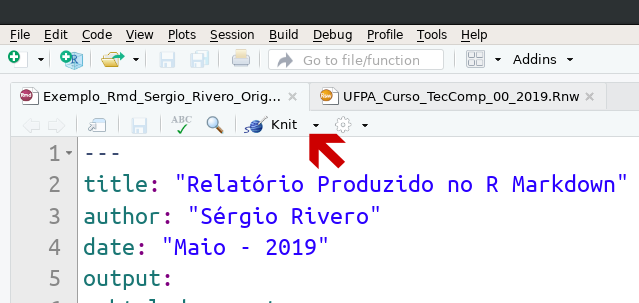
\includegraphics[width=0.7\linewidth]{../figs/BP_Curso_TecComp_00_2019_f04-02}
		\caption{O Botão Knit no Rstudio}
		\label{fig:bpcursoteccomp002019f04-02}
	\end{figure}
	
	
	A partir do arquivo .Rmd, você pode gerar resultados que combinem, textos, resultados de operações em R, tabelas geradas pelas bibliotecas do R (regressões, outras coisas), bem como gráficos. 
		\begin{figure}
		\centering
		\includegraphics[width=\linewidth]{../figs/BP_Curso_TecComp_00_2019_f04-01}
		\caption{O processo de geração de documentos no RMD}
		\label{fig:bpcursoteccomp002019f04-01}
	\end{figure}
	

	Estes programas permitem um caminho mais suave entre a análise e a publicação dos resultados.

	
	
	\section{A estrutura de um arquivo .Rmd}
	
	Um arquivo .Rmd tem basicamente, 3 partes.

	\begin{enumerate}
		\item 	Um cabeçalho escrito em YAML\footnote{YAML é um formato de serialização de dados legíveis por humanos inspirado em linguagens como XML, C, Python, Perl, assim como o formato de correio eletrônico especificado pela RFC 2822. YAML foi proposto por Clark Evans em 2001 em conjunto com Ingy döt Net e Oren Ben-Kiki (Wikipedia) - Mais informações em: \url{https://yaml.org/}}. Separados por "\verb|---|" ~no início e no final do bloco.
		\item Textos e comandos em Linguagem Markdown
		\item \textit{Chunks} em uma linguagem específica (no nosso casso, Comandos em R) - Separados por  "\verb|```|  " ~no início e no final do bloco.
	\end{enumerate}	 
	
	O cabeçalho (figura \ref{fig:bpcursoteccomp002019f04-04}) é posto uma vez e contém definições gerais do arquivo executado.  Há vários componentes do cabeçalho, sendo que os principais são o título, o nome do autor, a data e qual será a saída do arquivo executado (HTML, PDF, MSWord, etc)
	
	\begin{figure}
		\centering
		\includegraphics[width=0.7\linewidth]{../figs/BP_Curso_TecComp_00_2019_f04-04}
		\caption{Um exemplo de Cabeçalho de um arquivo .Rmd}
		\label{fig:bpcursoteccomp002019f04-04}
	\end{figure}
	

\section{Sintaxe de Markdown}

O texto em um documento R Markdown é gravado com a sintaxe Markdown. Precisamente falando, é o Markdown do Pandoc. Há muitos sabores de Markdown inventados por pessoas diferentes, e o sabor do Pandoc é o mais abrangente para o nosso conhecimento. Você pode encontrar a documentação completa do Markdown do Pandoc em \url{https://pandoc.org/MANUAL.html}. É altamente recomendável que você leia esta página pelo menos uma vez para conhecer todas as possibilidades com o Markdown da Pandoc, mesmo que você não use todas elas. Esta seção é adaptada da Seção 2.1 de Xie ( 2016 ) e abrange apenas um pequeno subconjunto da sintaxe Markdown do Pandoc.

\subsubsection{Formatação em linha}

O texto embutido será em itálico se estiver cercado por sublinhados ou asteriscos, por exemplo, \verb|_text_| ou \verb|*text*|. O texto em negrito é produzido usando um par de asteriscos duplos ( \verb|**text**|). Um par de tis (\verb|~~|) transformar texto para um subscrito (por exemplo, \verb|H~3~PO~4~|torna $H_3 PO_4$ ). Um par de circunflexos (\verb|^^|) produz um sobrescrito (por exemplo, \verb|Cu^2+^| renderiza $Cu^{2+}$).

Para marcar o texto como código \textit{inline}, use um par de backticks, por exemplo \verb|`code`|

Os hiperlinks são criados usando a sintaxe \verb|[text](link)|, por exemplo \verb|[RStudio](https://www.rstudio.com)|. 

A sintaxe das imagens é semelhante: basta adicionar um ponto de exclamação, por exemplo \verb|![alt text or image title](path/to/image)|, 

As notas de rodapé são colocadas dentro dos colchetes após um acento circunflexo \verb|^[]|, por exemplo \verb|^[This is a footnote.]|.


\subsubsection{Elementos de nível de bloco}

Cabeçalhos de seção podem ser escritos após um número de sinais de libra, por exemplo,

\verb|# First-level header|

\verb|## Second-level header|

\verb|### Third-level header|

Se você não quiser que um determinado título seja numerado, você pode adicionar \verb|{-}| ou \verb|{.unnumbered}| após o cabeçalho, por exemplo,

\verb|# Preface {-}|

Os itens da lista não ordenada começar com *, -ou +, e você pode aninhar uma lista dentro de outra lista pelo recuo da sub-lista, por exemplo,

- um item\\
- um item\\
- um item\\
~~~~- mais um item\\
~~~~- mais um item\\
~~~~- mais um item

A saída é:
\begin{itemize}
	\item um item
	\item um item
	\item um item
	\begin{itemize}
		\item mais um item
		\item mais um item
		\item mais um item
	\end{itemize}
\end{itemize}

Os itens da lista ordenada começam com números (você também pode aninhar listas dentro de listas), por exemplo,

1. o primeiro item\\
2. o segundo item\\
3. o terceiro item\\
~~~~~~- um item não ordenado\\
~~~~~~- um item não ordenado


A saída não parece muito diferente com a fonte Markdown:

\begin{enumerate}
	\item o primeiro item
	\item o segundo item
	\item o terceiro item
	\begin{itemize}
		\item um item não ordenado
		\item um item não ordenado
	\end{itemize}
\end{enumerate}



	
\section{Os \textit{chunks}}

	Um \textit{chunk} é uma parte de código (no nosso caso, R) incluído num arqivo \textbf{Rmarkdown}. Chunks iniciam com \verb|```{opcoes do chunk}| e terminam com \verb|```|. Na figura \ref{fig:bpcursoteccomp002019f04-05} podemos ver um exemplo de um chunk típico gerando um gráfico em R. 


	\begin{figure}[htpb]
		\centering
		\includegraphics[width=\linewidth]{../figs/BP_Curso_TecComp_00_2019_f04-05}
		\caption{Um \textit{chunk}}
		\label{fig:bpcursoteccomp002019f04-05}
	\end{figure}
	
	Algumas dicas importantes sobre as opções em um \textit{chunk} \footnote{O texto original pode ser encontrado em \url{https://yihui.name/knitr/options/}}:
	
	\begin{enumerate}
		\item Opções de \textit{chunk} devem ser escritas em uma linha; 
		\item não são permitidas quebras de linha dentro das opções de \textit{chunk};
		\item Evite espaços e pontos em rótulos de partes e nomes de diretórios; 
		\item Se sua saída for um documento TeX, esses caracteres podem causar problemas (em geral, é recomendável usar caracteres alfabéticos com palavras separadas por \verb|-| e evitar outros caracteres), por exemplo, \verb|setup-options| é um bom label, enquanto \verb|setup.options| e \verb|chunk 1| são ruins;
		\item Todos os valores de opções devem ser expressões R válidas, assim como escrevemos argumentos de função;
		\item para opções lógicas, deve-se usar \verb|TRUE| ou \verb|FALSE| ou \verb|T| ou \verb|F| mas, importante, "true" e "false"  não funcionam
	\end{enumerate}
	
	Abaixo falamos de algumas opções relevantes do cabeçalho de um chunk
	
	Primeiro o código pode ou não ser executado. O opção \verb|eval = FALSE| faz com que o código seja avaliado mas não executado. Sem nenhuma opção, o código é avaliado.
	
	Algumas opções que configuram os padrões de saída de um \textit{chunk} são:
	\begin{itemize}
		\item \textbf{echo:} (\verb|TRUE|) se deve incluir o código-fonte R no arquivo de saída; além de \verb|TRUE / FALSE| que liga / desliga completamente o código-fonte, também podemos usar um vetor numérico para selecionar quais expressões R ecoar em um trecho, por exemplo, \verb|echo = 2:3| significa apenas ecoar a segunda e terceira expressões, e \verb|echo = -4| significa excluir a quarta expressão;
		\item \textbf{results}: ('markup'; character) pega esses valores possíveis:
			\begin{itemize}
				\item \textbf{markup}: marque os resultados usando o gancho de saída, por ex. colocar resultados em um ambiente especial do \LaTeX;
				\item \textbf{asis}: saída como é, ou seja, grava os resultados brutos de R no documento de saída;
				\item \textbf{hold}: segura todas as saídas e as empurra para o final de um \textit{chunk}
				\item \textbf{hide}: oculta resultados.  esta opção só se aplica à saída R normal (não avisos, mensagens ou erros)				
			\end{itemize}
		\item \textbf{warning}: (default é VERDADEIRO;) preserva os avisos (produzidos por warning()) na saída como se executássemos código R em um terminal (se for  FALSO, todos os avisos serão impressos no console ao invés do documento de saída);
		\item \textbf{error}: (default é VERDADEIRO) preserva os erros (de stop()). A avaliação não será interrompida mesmo em caso de erros!! Se quisermos que R pare nos erros, precisamos definir essa opção como FALSO;
		\item \textbf{message}: (default é VERDADEIRO) preserva as mensagens emitidas por message() (semelhante ao warning).
	\end{itemize}

	Um detalhamento maior das opções de chunks no Rmarkdown podem ser achados em \url{https://yihui.name/knitr/options/}
	
	
	\section{Algumas referências sobre o Rmarkdown}
	
	\url{https://daringfireball.net/projects/markdown/}
	
	\url{https://rmarkdown.rstudio.com/authoring_quick_tour.html}
	
	\url{https://www.markdownguide.org/getting-started/}
	
	\url{https://ourcodingclub.github.io/2016/11/24/rmarkdown-1.html}
	
	\url{https://github.com/yihui/knitr-book}
	
	\url{https://www.rstudio.com/wp-content/uploads/2015/03/rmarkdown-reference.pdf}
	
	\url{https://www.rstudio.com/wp-content/uploads/2016/03/rmarkdown-cheatsheet-2.0.pdf}
	





%%%%%%%%%%%%%%%%%%%%%%%%%%%%%%%%%%%%%%%%%%%%%%%%%%%%%%%%%
%
%    CAPITULO
%
%%%%%%%%%%%%%%%%%%%%%%%%%%%%%%%%%%%%%%%%%%%%%%%%%%%%%%%%%
%
% !Rnw root = BP_Curso_TecComp_00_2019.Rnw


		
\chapter{Acessando e Utilizando Bases de Dados}

Apresentar o conceito de Dataframe, os tipos de dados utilizados no R e os principais comandos  

\section{O ciclo de tratamento e análise de dados}

Atividades que utilizam dados e fazem algum tratamento formal (estatístico, matemático) destes dados são comuns tanto no mundo acadêmico quanto no mundo corporativo. Muitas vezes, os dados correspondem a milhões de observações em diversas bases de dados. Estas bases de dados, muitas vezes têm estruturas complexas e diferentes formas de organização, armazenamento, codificação, mecanismos de busca, etc. Tratar e analisar estes dados exige planejamento, avaliação, organização, o que implica em uma atividade sistemática e no uso de ferramentas adequadas para a tarefa.

Um outro aspecto relevante também é que muitos dados podem ser analisados, usando técnicas, objetivos e/ou perspectivas diferentes. O que significa que os mesmos dados, coletados e tratados, podem ter um reuso para diferentes projetos e análises. Esta possibilidade de reuso torna ainda mais importante o seu tratamento e armazenamento sistematizado. 

Podemos então dizer que os dados tem um \textit{ciclo de vida} e este ciclo pode ser pensado como um conjunto de atividades que vão do planejamento de seu uso até a sua análise. Abaixo, na figura \ref{fig:f02-01}, apresentamos um exemplo de ciclo de vida que pode ser encontrado em  \url{https://www.dataone.org/data-life-cycle}


\begin{figure}[htpb]
	\centering
	\includegraphics[width=\linewidth]{../figs/BP_Curso_TecComp_00_2019_f02-01}
	\caption{O Ciclo de Tratamento e Análise de Dados}
	\label{fig:f02-01}
\end{figure}


Este ciclo de vida tem oito componentes:


O ciclo de vida dos dados DataONE possui oito componentes \footnote{\url{https://www.dataone.org/data-life-cycle}}:

\begin{itemize}
	\item Planejar: descrição dos dados que serão compilados e como os dados serão gerenciados e disponibilizados ao longo de sua vida útil
	\item Coletar: as observações são feitas manualmente, com sensores ou outros instrumentos ou os dados são adquiridos de instituições que os produzem
	\item Validar: a qualidade dos dados é assegurada por meio de verificações e checagens
	\item Descrever: os dados são descritos com precisão e detalhadamente usando os padrões de metadados apropriados
	\item Preservar: os dados são submetidos a um arquivo de longo prazo apropriado (ou seja, data center)
	\item Descobrir: dados potencialmente úteis são localizados e obtidos, juntamente com as informações relevantes sobre os dados (metadados)
	\item Integrar: dados de fontes diferentes são combinados para formar um conjunto homogêneo de dados que podem ser prontamente analisados
	\item Analisar: os dados são analisados
	
\end{itemize}

Algumas atividades de pesquisa podem usar apenas parte do ciclo de vida; por exemplo, um projeto envolvendo metanálise pode se concentrar nas etapas de Descobrir, Integrar e Analisar, enquanto um projeto focado na coleta e análise de dados primários pode ignorar as etapas de Descobrir e Integrar. Além disso, outros projetos podem não seguir o caminho linear descrito aqui, ou várias revoluções do ciclo podem ser necessárias. Além disso, alguns cientistas ou equipes (por exemplo, aqueles envolvidos em modelagem e síntese) podem criar novos dados no processo de descobrir, integrar, analisar e sintetizar os dados existentes.


\begin{figure}[htpb]
	\centering
	\includegraphics[width=\linewidth]{../figs/BP_Curso_TecComp_00_2019_f02-02}
	\caption{Tratamento de Dados Estatísticos}
	\label{fig:f02-02}
\end{figure}

Uma outra abordagem para o ciclo de vida, mais focada no tratamento de dados estatísticos para modelagem é a que podemos ter em \url{https://paulvanderlaken.com/2017/07/07/tidyverse-101-simplifying-life-for-users/}. Neste caso, estamos falando de dados já adquiridos e digitalizados de alguma forma. Então a fase de aquisição de dados é feita a partir da importação de dados já coletados. O trabalho de economistas, é, na sua maioria das vezes, feito a partir de dados secundários adquiridos de instituições de pesquisa. Neste caso, esta abordagem (Figura \ref{fig:f02-02}) é mais próxima do ciclo normalmente utilizado em análises de dados secundários.


\begin{figure}[htpb]
	\centering
	\includegraphics[width=0.7\linewidth]{../figs/BP_Curso_TecComp_00_2019_f02-03}
	\caption{Ferramentas de Tratamento de Dados em R}
	\label{fig:f02-03}
\end{figure}

Como podemos ver na figura \ref{fig:f02-03}, temos muitos pacotes para cada tipo de tratamento. A lista acima não é exaustiva. Muito provavelmente há mais pacotes que são especializados para a resolução de problemas mais específicos, como o acesso a bases de dados SQL ou a geração de páginas na internet para visualização ou o acesso a arquivos JSON ou YAML. Por isso, é importante sempre avaliar quais os pacotes mais adequados para a solução do seu problema de tratamento de dados.

 O \textit{readr}, por exemplo \footnote{\url{https://cran.r-project.org/web/packages/readr/index.html}} é um pacote genérico para dados em formato matricial (\textit{retangular data}), tais como arquivos csv, tsv, fwf. Para ler arquivos \textit{xls} e \textit{xlsx} há pacotes como o \textit{readxl} e o \textit{xlsx}\footnote{\url{https://cran.r-project.org/web/packages/readxl/index.html} e \url{https://cran.r-project.org/web/packages/xlsx/index.html}}


O tratamento dos dados pode facilmente consumir a maior parte do tempo de um projeto de análise e modelagem. A existência de ferramentas que facilitem esta tarefa e reduzam o tempo despendido nela é uma ajuda que vem bem a calhar.

Há no R um conjunto de pacotes feitos especialmente para a fase de tratamento dos dados. O \textit{tydiverse} \cite{Wickham2014} permite a redução dos erros de codificação e a construção de um código mais simples, claro e eficaz, resduzindo assim o tempo necessário para o tratamento e limpeza dos dados \footnote{\url{https://cran.r-project.org/web/packages/tidyr/vignettes/tidy-data.html}}


O \textit{tidyverse} tem  pacotes  que fornecem funcionalidades para executar eficazmente as atividades de tratamentos e análise de dados, reduzindo o esforço de codificação e a possibilidade de erros. 

A maioria das vezes neste tipo de cenário os dados estão armazenados em formatos externos ao R e devem ser importados\footnote{por exemplo, Excel, SPSS, Spyder, Jupyter}. 

Uma segunda etapa do trabalho é garantir a correção dos dados. Para isso é necessário "limpar" e "arrumar" os dados. Nesta fase é necessário eliminar erros, inconsistências de tipos de dados, problemas de codificação e representação dos dados e, eventualmente, gerar novas variáveis a partir dos próprios dados que sejam necessárias para a análise. Este processo é cíclico e também parte da análise. Durante o processo de análise dos dados é possível que surja a necessidade de novas variáveis ou que se descubra erros ainda existentes nos dados de entrada, o que implica em sua correção. 

O processo então continua até que se tenha o modelo suficientemente eficaz e testado para que resultados significativos possam ser comunicados.


Mas uma pergunta é, o que são dados limpos? Os dados limpos têm algumas características fundamentais:

\begin{enumerate}
	\item Cada coluna da sua base de dados tem apenas um tipo de dado e corresponde a apenas uma variável;
	\item Cada linha de sua base de dados corresponde a apenas uma observação;
	\item Cada elemento da base corresponde a um dado de uma variável em uma observação. 
	\item Preferencialmente, o número de observações faltantes é mínimo.
\end{enumerate}


Alguns dos pacotes utilizados para importar dados no R são:

\begin{itemize}
	\item \textit{haven} - para importar arquivos SPSS, Stata, e SAS;
	\item \textit{readxl} e \textit{xlsx} - arquivos excel (.xls e .xlsx);
	\item \textit{DBI} - arquivos de bancos de dados;
	\item \textit{jsonlite} - arquivos \textit{json};
	\item \textit{xml2} - arquivos padrão \textit{XML}
	\item \textit{httr} - \textit{APIs} na \textit{Web}
\end{itemize}

Há um conjunto grande de pacotes em R para importação de dados. O ideal é, na fase do planejamento do tratamento dos dados, você definir qual estratégia utilizar para importar os dados para o R.


\section{Tipos de Dados em R}

Os tipos de dados do R incluem: dados escalares, vetores, matrizes, listas e quadro de dados (Dataframe).

\begin{figure}
	\centering
	\includegraphics[width=\linewidth]{../figs/BP_Curso_TecComp_00_2019_f02-04}
	\caption{Uma representação gráfica dos tipos de dados em R. \\ Fonte: \url{http://venus.ifca.unican.es/Rintro/index.html}}
	\label{fig:f02-04}
\end{figure}



\subsection{Escalares}
Determinada variável pode ser um escalar, ou seja, simplesmente um número:

Exemplo de escalares:
\begin{Schunk}
\begin{Sinput}
> a <- 2
> b <- 2*a
> a
\end{Sinput}
\begin{Soutput}
[1] 2
\end{Soutput}
\begin{Sinput}
> b
\end{Sinput}
\begin{Soutput}
[1] 4
\end{Soutput}
\end{Schunk}

\subsection{Vetores}
O vetor é um objeto matemático caracterizado em um conjunto de segmentos orientdos de reta que possuem o mesmo módulo, direção e sentido. Ele contêm elementos de classes diferentes, conforme apresentado abaixo:


Vetor de classe numérica:
\begin{Schunk}
\begin{Sinput}
> a <- c(1,3500,5.3,543,-2,4000)
\end{Sinput}
\end{Schunk}
Vetor de classe de caractér:
\begin{Schunk}
\begin{Sinput}
> b <- c("taxa de juros","taxa de câmbio","reservas bancárias") 
\end{Sinput}
\end{Schunk}
Vetor de classe lógica:
\begin{Schunk}
\begin{Sinput}
> c <- c(FALSE,TRUE,FALSE,TRUE) 
\end{Sinput}
\end{Schunk}
\subsection{Matrizes}
São compostas por linhas (valores ordenados na horizontal) representadas pela letra "m" e colunas (valores ordenados na vertical) representadas pela letra "n", onde os dados são convertidos segundo essas disposições.
\begin{Schunk}
\begin{Sinput}
> matriz <- matrix(data=1:16,nrow=4,ncol=4)
> matriz
\end{Sinput}
\begin{Soutput}
     [,1] [,2] [,3] [,4]
[1,]    1    5    9   13
[2,]    2    6   10   14
[3,]    3    7   11   15
[4,]    4    8   12   16
\end{Soutput}
\end{Schunk}
Onde:
       \begin{description}
       \item [data:] parâmetro que representa os dados usados para criar matriz;
       \item [nrow:] parâmetro para número de linhas;
       \item [ncol:] parâmetro para número de colunas.
       \end{description}

\subsection{Array}

O dado pode ser um \textbf{Array}. Essa estrutura de dados possui três dimensões, as linhas, as colunas e as camadas. 

Exemplo de Array:
\begin{Schunk}
\begin{Sinput}
> cubo <- array(data = 1:27, dim=c(3,3,3))
> cubo
\end{Sinput}
\begin{Soutput}
, , 1

     [,1] [,2] [,3]
[1,]    1    4    7
[2,]    2    5    8
[3,]    3    6    9

, , 2

     [,1] [,2] [,3]
[1,]   10   13   16
[2,]   11   14   17
[3,]   12   15   18

, , 3

     [,1] [,2] [,3]
[1,]   19   22   25
[2,]   20   23   26
[3,]   21   24   27
\end{Soutput}
\end{Schunk}

       \begin{description}
       \item [data:] parâmetro que representa os dados usados para criar matriz;
       \item [dim:] parâmetro para determinar as dimensões do array, sendo \textbf{dim} um vetor;
       \end{description}

\url{https://www.statmethods.net/input/datatypes.html}

\url{https://swcarpentry.github.io/r-novice-inflammation/13-supp-data-structures/}

\url{https://www.tutorialspoint.com/r/r_data_types.htm}

\url{http://www.r-tutor.com/r-introduction/basic-data-types}

\url{https://www.cyclismo.org/tutorial/R/types.html}

\url{https://stat.ethz.ch/R-manual/R-devel/library/base/html/typeof.html}

\section{Dataframes}

Data frame é uma formatação de tabela presente no R que comporta duas dimensões. A primeira dimensão compreende as linhas(Observações) e a segunda dimensão compreende as colunas(variáveis). 

Vetor dos meses:
\begin{Schunk}
\begin{Sinput}
> DATA <- c("ago/2018", "set/2018", "out/2018", 
+           "nov/2018", "dez/2018", "jan/2019")
> DATA
\end{Sinput}
\begin{Soutput}
[1] "ago/2018" "set/2018" "out/2018" "nov/2018" "dez/2018" "jan/2019"
\end{Soutput}
\end{Schunk}

Vetor do IPCA para os respectivos meses do vetor DATA:
\begin{Schunk}
\begin{Sinput}
> IPCA <- c(-0.09, 0.48, 0.45, -0.21, 0.15, 0.32)
> IPCA
\end{Sinput}
\begin{Soutput}
[1] -0.09  0.48  0.45 -0.21  0.15  0.32
\end{Soutput}
\end{Schunk}

Vetor do Pib mensal em milhões(R\$) para os respectivos meses do vetor DATA:
\begin{Schunk}
\begin{Sinput}
> PIBmensalMilhoes <- c(583011.3, 551215.6, 597218.7,
+                       604073.9, 624464.1, 591715.7)
> PIBmensalMilhoes
\end{Sinput}
\begin{Soutput}
[1] 583011.3 551215.6 597218.7 604073.9 624464.1 591715.7
\end{Soutput}
\end{Schunk}

\newpage

Unimos os três vetores criados anteriormente em uma única estrutura de dados e conseguinte transformamos essa estrutura em um dataframe por meio dos comandos a baixo:
\begin{Schunk}
\begin{Sinput}
> Dados <- data.frame(cbind(DATA, IPCA, PIBmensalMilhoes))
> Dados
\end{Sinput}
\begin{Soutput}
      DATA  IPCA PIBmensalMilhoes
1 ago/2018 -0.09         583011.3
2 set/2018  0.48         551215.6
3 out/2018  0.45         597218.7
4 nov/2018 -0.21         604073.9
5 dez/2018  0.15         624464.1
6 jan/2019  0.32         591715.7
\end{Soutput}
\end{Schunk}



\url{https://www.tutorialspoint.com/r/r_data_frames.htm}

\url{https://www.datamentor.io/r-programming/data-frame/}

\url{http://www.r-tutor.com/r-introduction/data-frame}

\url{https://stat.ethz.ch/R-manual/R-devel/library/base/html/data.frame.html}

\url{https://www.tutorialgateway.org/data-frame-in-r/}

\url{https://datacarpentry.org/R-ecology-lesson/02-starting-with-data.html}

\url{https://www.statmethods.net/input/importingdata.html}

\section{Acessando Arquivos no computador}

Para acessar um conjunto de documentos e manusear seus dados no R, primeiramente salve o arquivo no computador ou então obtenha os dados através da internet ou outras fontes. Importante prestar atenção quanto ao tipo de arquivo que se esta trabalhando, pois a prática de importar os dados para o R requer uma própria função a depender do tipo de arquivo, que pode ser: HTML, XML, Json, dados espaçados por TAB, linhas de arquivo de texto, HDF5, SPSS, Stata e outros, com inúmeros tutoriais disponíveis a pesquisa para mais informações, ficando este material no enfoque da apresentação de dois formatos de arquivos que são bastante utilizados: o csv e o xlsx..

\subsection{Importando arquivo CSV (Comma separated values) em R}


Ao salvar um arquivo em formato csv, execute o comando abaixo no R:

\begin{Schunk}
\begin{Sinput}
> MyData <- read.csv(file="aux/PIB_BR_1996-2016.csv", header=TRUE, sep=",")
\end{Sinput}
\end{Schunk}

Onde:

file = Parâmetro que representa o arquivo que se vai importar no R. 

Observação: Copie e cole o arquivo ou endereço, conforme o exemplo, que vai ser lido em um quadro de dados chamado MyData

header = Parâmetro que especifica que esses dados incluem uma linha de cabeçalho.
 
 Observação: no trabalho com planilhas, a primeira linha é geralmente reservada para o cabeçalho.

sep = Parâmetro de indicativo que os dados vão ser separados, neste caso, por vírgulas, pois arquivos separados por vírgulas são mais fáceis de trabalhar.

Observação: em seu conjunto de dados evite nomes,valores ou campos com espaços em branco, pois cada palavra será interpretada como uma variável separada, o que resulta em erros relacionados ao número de elementos por linha em seu conjunto de dados. Para concatenar palavras insira . entre as palavras em vez de espaço. Nomes curtos são mais adequados em nomes mais longos. Evitar nomes que contenham símbolos como os seguintes: (\verb+$%^&*()-#?<>/|\[]{}+). Estes símbolos não poderão ser utilizados.

\section{Importando arquivo xlsx em R  }

Ao salvar um arquivo em formato xlsx, execute os comandos abaixo no R:

\begin{Schunk}
\begin{Sinput}
> library(xlsx)
> xlsxFile = "aux/PIB_BR_1996-2016.xlsx"
> myFile = read.xlsx(xlsxFile, 1, rowIndex = 1)
\end{Sinput}
\end{Schunk}

Onde:

xlsxFile = Parâmetro que representa o arquivo xlsx, objeto de pasta de trabalho ou URL para o arquivo xlsx.

o segundo parâmetro é o número da planilha que você vai importar

o parâmetro "rowIndex", indica onde você vai começar a ler o arquivo.

A documentação do pacote está em: \url{https://cran.r-project.org/web/packages/xlsx/xlsx.pdf}

\subsection{Mais informações}

Informações mais detalhadas sobre importação de dados, podem

\url{https://www.datacamp.com/community/tutorials/r-data-import-tutorial?utm_source=adwords_ppc&utm_campaignid=1455363063&utm_adgroupid=65083631748&utm_device=c&utm_keyword=&utm_matchtype=b&utm_network=g&utm_adpostion=1t1&utm_creative=332602034364&utm_targetid=dsa-473406573035&utm_loc_interest_ms=&utm_loc_physical_ms=1001610&gclid=Cj0KCQiA5NPjBRDDARIsAM9X1GLkgYWekNMkjHQnsTnRAzV7_gVEiwAqyW9CPisvAqFv2mNXzwarSlIaAgdZEALw_wcB}

\url{http://rprogramming.net/read-csv-in-r/}

\url{https://www.rdocumentation.org/packages/gdata/versions/2.18.0/topics/read.xls}

\url{https://stat.ethz.ch/R-manual/R-devel/library/utils/html/read.fwf.html}

\url{https://riptutorial.com/r/example/31447/importing-fixed-width-files}


\section{Acessando Bases de dados via \textit{APIs}}


APIs são abreviatura para Application Programming Interface (Interface de Programação de Aplicativos), permite à máquina o acesso à funcionalidade do programa dentro de outro programa, realizando a açãoodo programa automaticamente, para o uso de funcionalidades e leitura de dados.


\subsection{Pacotes Obrigatórios}

O acesso a APIs em R, pode ser feito com o pacote httr \footnote{produzido po Hadley Wickham - \url{http://hadley.nz/}} atua criando chamadas de APIs e lidando com autenticação destas;

O pacote jsonlite, realiza suporte ao trabalho com dados JASON, para traduzir as estruturas de dados aninhadas do JSON em objetos R sensíveis; 

O  pacote lubridate, atua na transformação e extração de datas, funções úteis para trabalhar com datas, fusos horá¡rios e operações aritméticas com datas; 
\url{http://material.curso-r.com/lubridate/}


Para obtê-los 

\textbf{install.packages(c("httr", "jsonlite", "lubridate"))}


Carregar os pacotes


A funcionalidade do R em transformar automaticamente as cadeias de caracteres em variáveis de fator (de utilidade estatística), opera de maneira indesejada,e deverá ser efetuada uma chamada de desligamento (que atuará somente nesta sessão e depois retornará à funcionalidade anterior quando reiniciado, o R). 



Argumentos de consulta:
\begin{itemize}
	\item GET(): Recupera o arquivo;
	\item POST(): Adiciona um arquivo;
	\item DELETE(): Remove um arquivo;
	
\end{itemize}

\begin{enumerate}
	\item As API's possuem estruturas de solicitação, para isso uma solicitação de HTTP referente à base de dados com que será trabalhada, segue as seguintes descrições:
	\begin{enumerate}
		\item Verbo HTTP ( GET, POST, DELETE, etc.);
		\item O URL base da API;
		\item O caminho da URL ou o endpoint;
		\item Argumentos de consulta de URL (por exemplo, ?foo=bar);
		\item Cabeçalhos opcionais;
		\item Um corpo de solicitação opcional;
	\end{enumerate}
	
	\item usa-se a função download.file() para baixar um arquivo para o seu computador e trabalhar com ele mantendo salva uma cópia dos dados no seu computador).
	
	\item É necessário fazer analise a saída em um objeto R. podendo verificar O pacote que realiza suporte ao trabalho com dados JASON (para traduzir as estruturas de dados JSON em objetos R),faça a intalação do pacote jasolite.
	
	\item Em seguida use a função fromJSON() no pacote rjson para importar esses dados para um objeto data.frame."
	
	\item Com os dados em um formato data.frame, é possível limpá-los. 
	
	
\end{enumerate}

Exemplo de base de dados JASON retirada do Banco Central do Brasil:

Instala o pacote (apenas uma vez)

install.packages("jsonlite")

Comando para fazer o download

download.file("http://api.bcb.gov.br/dados/serie/bcdata.sgs.4329/dados?formato=json\&amp;dataInicial=01/01/2001","ICMS")

\begin{Schunk}
\begin{Sinput}
> library(jsonlite)
> ICMS_json <- jsonlite::fromJSON("ICMS")
> ICMS <- as.data.frame(ICMS_json)
> ICMS$valor <- as.numeric(ICMS$valor)
> str(ICMS)
> ICMS$data <- as.Date(ICMS$data)
> str(ICMS)
> download.file("http://api.bcb.gov.br/dados/serie/bcdata.sgs.433/dados?formato=json&amp;dataInicial=01/01/2001","IPCA")
> IPCA <- jsonlite::fromJSON("IPCA")
> as.numeric(IPCA[,2])
> ICMS <- ICMS[31:325,]
> IPCA <- IPCA[175:469,]
> IPCA <- IPCA[,2]
> IPCA_new <- as.numeric(IPCA)
> IPCA <- IPCA_new
> IPCS_new <- NULL
> data <- cbind(ICMS, IPCA)
> deflator <- as.numeric(data[295,3])
> VR <- (deflator/(as.numeric(data[,3])))*data[,2]
> plot.ts(VR)
\end{Sinput}
\end{Schunk}

\url{https://www.r-bloggers.com/accessing-apis-from-r-and-a-little-r-programming/}

\url{https://cran.r-project.org/web/packages/httr/vignettes/api-packages.html}

\url{https://zapier.com/learn/apis/}

\url{https://www.earthdatascience.org/courses/earth-analytics/get-data-using-apis/API-data-access-r/}



\section{Trabalhando com bases de dados muito grandes}

\url{http://dept.stat.lsa.umich.edu/~jerrick/courses/stat701/notes/sql.html}

\url{https://datacarpentry.org/R-ecology-lesson/05-r-and-databases.html}

\url{https://db.rstudio.com/}

\url{http://www.columbia.edu/~sjm2186/EPIC_R/EPIC_R_BigData.pdf}

\url{https://www.rstudio.com/resources/webinars/working-with-big-data-in-r/}

\url{https://rpubs.com/msundar/large_data_analysis}









%%%%%%%%%%%%%%%%%%%%%%%%%%%%%%%%%%%%%%%%%%%%%%%%%%%%%%%%%
%
%    CAPITULO
%
%%%%%%%%%%%%%%%%%%%%%%%%%%%%%%%%%%%%%%%%%%%%%%%%%%%%%%%%%
%
% !Rnw root = BP_Curso_TecComp_00_2019.Rnw


\chapter{Limpando e organizando seus dados}

	\section{O que é uma boa base de dados e que tipos de bases existem?}
	Boas bases de dados para trabalhar, sobretudo com tidy, são bases que possuem variáveis nas colunas e observações nas linhas. 
	Podemos identificar tal estrutura na figura \ref{fig:f03-01}  abaixo:
	
\begin{figure}[htpb!]
	\centering
	\includegraphics[width=\linewidth]{../figs/BP_Curso_TecComp_00_2019_f03-01}
	\caption{Organização ideal para base de dados}
	\label{fig:f03-01}
\end{figure}

Há três tipos bases de dados principais que comportam a estrutura de variáveis nas colunas e observações nas linhas que são:

\begin{itemize}
	\item Séries Temporais
	\item Cortes Transversais
	\item Dados em Painel
\end{itemize}

\subsection{Série Temporal}

Séries temporais(ou longitudinais) são identificadas como observações ordenadas ao longo do "tempo". Exemplos:
\begin{itemize}
\item PIB distribuído anualmente;
\item Arrecadação mensal de um ou mais Estados;
\item Taxa de câmbio diária.
\end{itemize}

Um bom exemplo de fonte de bases de dados de series temporais é o SGS - Banco Central. Segue o link abaixo:

\url{https://www3.bcb.gov.br/sgspub/localizarseries/localizarSeries.do?method=prepararTelaLocalizarSeries}


\begin{figure}[htpb]
	\centering
	\includegraphics[width=\linewidth]{../figs/BP_Curso_TecComp_00_2019_f03-02}
	\caption{Exemplo de série temporal}
	\label{fig:f03-02}
\end{figure}

\subsection{Corte Transversal}

Dados transversais(ou cross-section) são identificados quando não há importância de ordenação das observações, além de representar dados em um único ponto do "tempo". Exemplos:

\begin{itemize}
\item Arrecadação de ICSM para todos Estados do Brasil para o ano de 2018;
\item Dados demográficos para todos os municípios do Pará para o ano de 2010.
\end{itemize}

Um bom exemplo de fonte de bases de dados de cortes transversais é o Sidra - IBGE. Segue o link abaixo:

\url{https://sidra.ibge.gov.br/home}


\begin{figure}[htpb!]
	\centering
	\includegraphics[width=\linewidth]{../figs/BP_Curso_TecComp_00_2019_f03-03}
	\caption{Base de dados de Série Temporal}
	\label{fig:bpcursoteccomp002019f03-03}
\end{figure}


\begin{Schunk}
\begin{Sinput}
>  library(dplyr)
\end{Sinput}
\end{Schunk}

  Nesta seção utilizaremos a base de dado "starwars", que é uma base nativa do pacote dplyr. Para que possamos ter acesso a base, devemos utilizar a função a seguir:
  
\begin{Schunk}
\begin{Sinput}
> data("starwars")
\end{Sinput}
\end{Schunk}
  
  \subsection{Funções de Remodelagem}
A primeira função apresentada é a função \textbf{arrange}, que consiste em ordenar uma coluna(variável) de forma crescente ou decrescente. As função é escrita da seguinte forma:

\begin{Schunk}
\begin{Sinput}
> starwars11 <- arrange(starwars, mass) #Para ordenamento crescente
> starwars12 <- arrange(starwars, desc(height)) #Para ordenamento decrescente
\end{Sinput}
\end{Schunk}
  
Estão apresentadas a seguir as funções utilizadas para renomear rótulos(nomes) de colunas(variáveis).

\begin{Schunk}
\begin{Sinput}
> starwars21 <- rename(starwars, nome = name)
> starwars22 <- rename(starwars, altura = height)
> starwars23 <- rename(starwars, massa = mass)
\end{Sinput}
\end{Schunk}

\subsection{Funções de Filtragem}
A função \textbf{filter} extrai linhas de uma base de dados a partir de um critério lógico. Essa função é bastante útil quando é preciso extrair um conjunto de dados que apresentam determinadas características. Por exemplo quando é preciso criar um novo objeto sem os outliers. A função está descrita abaixo:

\begin{Schunk}
\begin{Sinput}
> starwars31 <- filter(starwars, mass < 70)
\end{Sinput}
\end{Schunk}

A função \textbf{distinct} remove todas as linhas que se encontram duplicadas na base de dados, permanecendo apenas uma de cada linha duplicada. Utilizamos a função da seguinte forma:

Observação: Para que possamos usar a função \textbf{distinct}, criamos o objeto \emph{starwars32} com as linhas 31 até a 60 duplicadas.

\begin{Schunk}
\begin{Sinput}
> starwars32 <- rbind(starwars, starwars[31:60,])
> starwars32 <- distinct(starwars32)
\end{Sinput}
\end{Schunk}

A função \textbf{sample\_frac} seleciona aleatoriamente o número de linhas correspondentes a fração determinada na função. O exemplo abaixo seleciona aleatoriamente 40\% das linhas da base de dados.

\begin{Schunk}
\begin{Sinput}
> starwars41 <- sample_frac(starwars, 0.4, replace = TRUE)
\end{Sinput}
\end{Schunk}

A função \textbf{sample\_n} seleciona um número $N$ de linhas. Onde $N$ é o número de linhas que devem ser extraídas.
\begin{Schunk}
\begin{Sinput}
> starwars42 <- sample_n(starwars, 25, replace = TRUE)
\end{Sinput}
\end{Schunk}

A função \textbf{slice} extrai linhas de acordo com as posições das linhas. Para o exemplo abaixo, criamos um novo objeto com as linhas 10 até a linha 50.


A função \textbf{select} seleciona colunas a partir dos rótulos especificados na função.

\begin{Schunk}
\begin{Sinput}
> starwars61 <- select(starwars, name, height, mass)
> starwars62 <- select(starwars, name, gender, species)
\end{Sinput}
\end{Schunk}

Para combinação de duas ou mais bases de dados temos as funções de \textbf{"join"}. A primeira é a função \textbf{left\_join} que insere uma base de dados a outra pela esquerda. 

\begin{Schunk}
\begin{Sinput}
> starwars71 <- left_join(starwars61, starwars62, by = "name")
\end{Sinput}
\end{Schunk}

A função \textbf{right\_join} insere uma base a outra pela direita.

\begin{Schunk}
\begin{Sinput}
> starwars72 <- right_join(starwars61, starwars62, by = "name")
\end{Sinput}
\end{Schunk}

A função \textbf{full\_join} insere uma base a outra a partir de uma chave comum nas duas bases.

\begin{Schunk}
\begin{Sinput}
> starwars73 <- full_join(starwars61, starwars62, by = "name")
\end{Sinput}
\end{Schunk}

Além de todas essas funções apresentadas anteriormente, o dplyr permite concatenar funções por meio de um mecanismo chamado \textbf{pipe}. Para utilizar o pipe é preciso colocar tais símbolos: 

\begin{itemize}
	\item \%>\%
\end{itemize}

Abaixo temos um exemplo da utilização do pipe. O exemplo consiste em calcular média e desvio padrão a partir de um agrupamento por espécie da base de dados starwars.

\begin{Schunk}
\begin{Sinput}
> starwars81 <- starwars %>%
+   group_by(species) %>%
+   summarise(desvpad = sd(birth_year, na.rm = TRUE),
+             avg = mean(birth_year, na.rm = TRUE))
\end{Sinput}
\end{Schunk}

\section{tidyr}

\textbf{Tidyr} é um pacote de tratamento de dados que fornece funções baseadas na organização de observações nas linhas e variáveis nas colunas, além de possuir boa relação com outros pacotes, como o \textbf{dplyr} para tratamento de dados e \textbf{ggplot} para apresentação de resultados.
	
A fonte para parte das figuras desta seção está em \url{https://github.com/rstudio/cheatsheets/blob/master/data-import.pdf}
	
	
Para utilizar o pacote precisamos efetuar a instalação do pacote e depois executar o mesmo.

\begin{Schunk}
\begin{Sinput}
> install.packages("tidyr")
\end{Sinput}
\end{Schunk}


\begin{Schunk}
\begin{Sinput}
> library(tidyr)
\end{Sinput}
\end{Schunk}
Para os exemplos desta seção utilizaremos as bases de dados \textbf{population} e \textbf{table2} do próprio tidyr. Para utilizar as duas bases precisamos efetuar dois comandos, que são:

\begin{Schunk}
\begin{Sinput}
> data("population")
> data("table2")
\end{Sinput}
\end{Schunk}

O \textbf{tidyr} possui quatro funções de remodelagem que são:

	
\subsection{Gather}	
A função \textbf{gather} é oposta a função \textbf{spread}, visto que \textbf{gather} transforma os rótulos das variáveis(nome das colunas) em observações(linhas). Para tal exemplo utilizaremos a base de dados \textbf(table2).

Primeiro transformaremos o fator(cases, count) em colunas.

\begin{Schunk}
\begin{Sinput}
> View(table2)
> population12 <- table2 %>% spread(type, count) 
> View(population12)
\end{Sinput}
\end{Schunk}

	
\begin{figure}[htpb]
	\centering
	\includegraphics[width=.6\linewidth]{../figs/BP_Curso_TecComp_00_2019_f03-04.png}
	\caption{Exemplo da função gather: gather(table4a, `1999`, `2000`,key = "year", value = "cases")}
	\label{fig:bpcursoteccomp002019f03-04}
\end{figure}

Depois retornaremos com o fator(cases, count) para as linhas, retornando ao painel de dados anteriormente.

\begin{Schunk}
\begin{Sinput}
> population13 <- population12 %>% gather(type, count, cases:population)
> View(population13)
\end{Sinput}
\end{Schunk}
	

\subsection{Spread}
A função \textbf{spread} transforma linhas em colunas. É bastante útil quando é preciso transformar dados categóricos em variáveis.

No exemplo abaixo transformamos um painel de dados em uma série temporal, sendo as variáveis os países presentes na base de dados \textbf{population}.

\begin{Schunk}
\begin{Sinput}
> View(population)
> population11 <- population %>% spread(country, population)
> View(population11)
\end{Sinput}
\end{Schunk}


	
\begin{figure}[htpb]
	\centering
	\includegraphics[width=.6\linewidth]{../figs/BP_Curso_TecComp_00_2019_f03-05.png}
	\caption{Exemplo da função spread: spread(table2, type, count)}
	\label{fig:bpcursoteccomp002019f03-05}
\end{figure}


\newpage
\subsection{Unite}

A função \textbf{unite} agrega o conteúdo de todas as linhas de duas colunas distintas em uma única coluna. Para o exemplo dessa função utilizaremos o dataset \textbf{table1} para unir o conteúdo de duas colunas.

Primeiramente acessamos o dataset \textbf{table1}:

\begin{Schunk}
\begin{Sinput}
> data("table1")
> head(table1)
\end{Sinput}
\end{Schunk}

Após ter acesso ao dataset, podemos executar a função \textbf{unite} para juntar os conteúdos \textbf{country} e \texttt{year} em uma única coluna. Fazemos a ação da seguinte forma:

\begin{Schunk}
\begin{Sinput}
> table2 <- unite(table1, "country_year", c("country","year"))
> head(table2)
\end{Sinput}
\end{Schunk}

\begin{figure}[htpb]
	\centering
	\includegraphics[width=.6\linewidth]{../figs/BP_Curso_TecComp_00_2019_f03-06.png}
	\caption{Exemplo da função unite: unite(table5, century, year,
		col = "year", sep = ``""``)}
	\label{fig:bpcursoteccomp002019f03-06}
\end{figure}	
	
	
\subsection{Separate}

A função \textbf{separate} desagrega o conteúdo de uma coluna em duas novas colunas. Para o exemplo dessa função utilizaremos o dataframe \textbf{table2} criado no exemplo anterior.

A função de seperação é a seguinte:

\begin{Schunk}
\begin{Sinput}
> table3 <- separate(table2, country_year, c("country", "year"), sep = "_")
> head(table3)
\end{Sinput}
\end{Schunk}

Como resultado da separação é preciso que obtenhamos um dataframe \textbf{table3} exatamente igual ao dataframe \textbf{table1}. Para checarmos o resultado está conforme o esperado, podemos executar o respectivo comando:

\begin{Schunk}
\begin{Sinput}
> table3 == table1
\end{Sinput}
\end{Schunk}

\begin{figure}[htpb]
	\centering
	\includegraphics[width=.6\linewidth]{../figs/BP_Curso_TecComp_00_2019_f03-07.png}
	\caption{Exemplo da função separate: separate(table3, rate,
		into = c("cases", "pop"))}
	\label{fig:bpcursoteccomp002019f03-07}
\end{figure}






\begin{figure}[htpb]
	\centering
	\includegraphics[width=.6\linewidth]{../figs/BP_Curso_TecComp_00_2019_f03-08.png}
	\caption{Exemplo da função separate\_rows: separate\_rows(table3, rate)}
	\label{fig:bpcursoteccomp002019f03-08}
\end{figure}




\subsection{Lidando com valores omissos}


\begin{figure}[htpb]
	\centering
	\includegraphics[width=.5\linewidth]{../figs/BP_Curso_TecComp_00_2019_f03-09.png}
	\caption{Exemplo da função drop\_na: drop\_na(x, x2)}
	\label{fig:bpcursoteccomp002019f03-09}
\end{figure}



\begin{figure}[htpb]
	\centering
	\includegraphics[width=.5\linewidth]{../figs/BP_Curso_TecComp_00_2019_f03-10.png}
	\caption{Exemplo da função fill: fill(x,x2)}
	\label{fig:bpcursoteccomp002019f03-10}
\end{figure}




\begin{figure}[htpb]
	\centering
	\includegraphics[width=.5\linewidth]{../figs/BP_Curso_TecComp_00_2019_f03-11.png}
	\caption{Exemplo da função replace\_na: replace\_na(x, list(x2 = 2))}
	\label{fig:bpcursoteccomp002019f03-11}
\end{figure}




%%%%%%%%%%%%%%%%%%%%%%%%%%%%%%%%%%%%%%%%%%%%%%%%%%%%%%%%%
%
%    CAPITULO
%
%%%%%%%%%%%%%%%%%%%%%%%%%%%%%%%%%%%%%%%%%%%%%%%%%%%%%%%%%
%
% !Rnw root = BP_Curso_TecComp_00_2019.Rnw



\chapter{Gráficos em R}

	\section{ggplot}
	O pacote \textbf{ggplot2} é uma ferramenta de visualização gráfica bastante útil para apresentação de dados com muitos componentes. A estrutura de construção de gráficos utilizando o ggplot2 é basicamente definir os dados a serem plotados e o sistema de coordenadas. Uma boa forma de entender como funciona o \textbf{ggplot2} é por meio da metáfora de camadas. Cada detalhe do gráfico é uma camada de comando definido a partir das camadas principais(dados e coordenadas).
	
	A figura \ref{fig:f06-01} mostra cada camada do processo de construção de gráficos utilizando o ggplot2 
	
	\begin{figure}[htpb]
		\centering
		\includegraphics[width=0.7\linewidth]{../figs/BP_Curso_TecComp_00_2019_f06-01}
		\caption{Camadas do ggplot2}
		\label{fig:f06-01}
	\end{figure}

Abaixo estão as descrições de cada camada da figura \ref{fig:f06-01}

\begin{description}
	\item [Data:] Base de dados que será utilizada;
	\item [Asthetics:] Definição do conjunto de dados que a comporão o gráfico, bem como a posição de cada dado;
	\item [Scale:] Difinição dos escala dos valores do gráfico;
	\item [Objeto Geométrico:] Definição da geometria do gráfico;
	\item [Statistics:] Estatística descritiva dos dados utilizados para gerar o gráfico;
	\item [Facets:] Criação de subplots(divisão da janela de plots);
	\item [Sistema de Coordenada:] Definição do sistema de coordenadas.
\end{description}

Para os exemplos do pacote \textbf{ggplot2} utilizaremos o dataset Iris. Essa base de dados possui 5 variáveis que são:

\begin{description}
	\item [Sepal.Length:] Comprimento da sépala;
	\item [Petal.Length:] Comprimento da pétala;
	\item [Sepal.Width:] Largura da sépala;
	\item [Petal.Width:] Largura da pétala;
	\item [Species:] Espécias da plantas. 
\end{description}

\begin{Schunk}
\begin{Sinput}
> data("iris")
> head(iris)
\end{Sinput}
\begin{Soutput}
  Sepal.Length Sepal.Width Petal.Length Petal.Width Species
1          5.1         3.5          1.4         0.2  setosa
2          4.9         3.0          1.4         0.2  setosa
3          4.7         3.2          1.3         0.2  setosa
4          4.6         3.1          1.5         0.2  setosa
5          5.0         3.6          1.4         0.2  setosa
6          5.4         3.9          1.7         0.4  setosa
\end{Soutput}
\end{Schunk}

O primeiro gráfico apresentará a relação entre o comprimento da pétala e da sépala como pode ser visto na figura \ref{fig:f06-04}.


\begin{figure}[htpb]
	\centering
	\includegraphics[width=0.7\linewidth]{../figs/BP_Curso_TecComp_00_2019_f06-04}
	\caption{Relação de pontos entre os comprimentos Pétala e Sépala}
	\label{fig:f06-04}
\end{figure}

\newpage

Os comandos para gerar o gráfico são:

\begin{Schunk}
\begin{Sinput}
> g1 <- ggplot(iris, aes(x = Sepal.Length, y = Petal.Length)) + 
+ geom_point() +
+ ggtitle("Relação entre tamanho da Pétala e o tamanho da Sépala") +
+ labs(x="Tamanho da Sépala", y="Tamanho da Pétala")
> plot(g1)
\end{Sinput}
\end{Schunk}

O objeto \textbf{g1} recebe a função que trata do acesso a base aos dados \textbf{iris} e a definição da posição das variáveis. Tal função está descrita abaixo:

\begin{Schunk}
\begin{Sinput}
> g1 <- ggplot(iris, aes(x = Sepal.Length, y = Petal.Length))
> #iris indica a base de dados e aes() indica a posição das variáveis
\end{Sinput}
\end{Schunk}

 próxima camada indica qual é a geometria do gráfico. Tal função é dada por:

\begin{Schunk}
\begin{Sinput}
> geom_point()
\end{Sinput}
\end{Schunk}

As próximas camadas apresentam apenas títulos e legendas presentes nos gráficos, além da função plot para apresentar o gráfico na região de plot do \textbf{Rstudio}

\begin{Schunk}
\begin{Sinput}
> ggtitle("Relação entre tamanho da Pétala e o tamanho da Sépala") +
+ labs(x="Tamanho da Sépala", y="Tamanho da Pétala")
> plot(g1)
\end{Sinput}
\end{Schunk}

É possível incluir mais de uma geometria no gráfico.

\begin{figure}[htpb]
	\centering
	\includegraphics[width=0.7\linewidth]{../figs/BP_Curso_TecComp_00_2019_f06-05}
	\caption{Relação de comprimento entre Pétala e Sépala}
	\label{fig:f06-05}
\end{figure}

Para fazer o gráfico da figura \ref{fig:f06-05} podemos utilizar os comandos abaixo:

\begin{Schunk}
\begin{Sinput}
> g2 <- ggplot(iris, aes(x = Sepal.Length, y = Petal.Length)) + 
+ geom_point() +
+ geom_smooth() +
+ ggtitle("iris") +
+ labs(x="Sepal length", y="Petal Length")
> plot(g2)
\end{Sinput}
\end{Schunk}

Podemos fazer uma separação por variáveis categóricas e apresentá-las com cores distintas. Na \textbf{aes()} adicionamos o parâmetro $color = Species$. Para o nosso exemplo, a variável categórica é \textbf{Species}.

\begin{figure}[htpb!]
	\centering
	\includegraphics[width=0.7\linewidth]{../figs/BP_Curso_TecComp_00_2019_f06-06}
	\caption{Relação de comprimento e largura das Sépalas}
	\label{fig:f06-06}
\end{figure}


O exemplo para construir a figura \ref{fig:f06-06} está exemplificado abaixo:

\begin{Schunk}
\begin{Sinput}
> g3 <- ggplot(iris, aes(x = Sepal.Length, y = Sepal.Width, color = Species)) + 
+ geom_point() +
+ ggtitle("Relação entre comprimento e largura das sépalas por espécie") +
+ labs(x="Comprimento da Sépala", y="Largura da Sépala", color = "Espécie")
> plot(g3)
\end{Sinput}
\end{Schunk}

Podemos incluir mais uma camada e criar vários ambientes de plot dividindo o ambiente principal. Para que isso seja possível utilizaremos a função \textbf{facet.wrap()}.

\begin{figure}[htpb!]
	\centering
	\includegraphics[width=0.7\linewidth]{../figs/BP_Curso_TecComp_00_2019_f06-07}
	\caption{Relação entre comprimento e largura das sépalas por espécie}
	\label{fig:f06-07}
\end{figure}

O código para gerar o gráfico da figura \ref{fig:f06-07} está exposto abaixo:

\begin{Schunk}
\begin{Sinput}
> gf4 <- ggplot(iris, aes(x = Sepal.Length, y = Sepal.Width, color = Species)) + 
+ geom_point() +
+ facet_wrap(~Species) +
+ ggtitle("Relação entre o comprimento e a largura das sépalas") +
+ labs(x="Comprimento da Sépala", y="Largura da Sépala", color = "Espécie")
> plot(gf4)
\end{Sinput}
\end{Schunk}

\newpage

Percebam que na figura \ref{fig:f06-07} utilizamos a mesma variável para o parâmetro \textbf{color} e para o parâmetro \textbf{facet\_wrap}. Em um novo exemplo usando a base de dados \textbf{mpg}, utilizaremos os dois parâmetros citados anteriormente, mas com variáveis distintas para cada um.

\begin{figure}[htpb!]
	\centering
	\includegraphics[width=0.7\linewidth]{../figs/BP_Curso_TecComp_00_2019_f06-08}
	\caption{Autonomia de combustível de veículos}
	\label{fig:f06-08}
\end{figure}

O código que gera a figura \ref{fig:f06-08} está escrito abaixo:

\begin{Schunk}
\begin{Sinput}
> gf8 <- ggplot(mpg, aes(x = cty, y = hwy, color = class)) + 
+ geom_point() +
+ geom_line() +
+ facet_wrap(~manufacturer) +
+ ggtitle("Autonomia de combustível por Companhia e modelo de veículo") +
+ labs(x="Milhas por galão na cidade", y="Milhas por galão na estrada")
> plot(gf8)
\end{Sinput}
\end{Schunk}

É possível adicionar os tamanhos dos pontos pra indicar o impacto de outra variável. Para fazer isso basta adicionar uma camada na função \textbf{geom\_point(size $=$ cyl)}. O código fica da seguinte forma:

\begin{Schunk}
\begin{Sinput}
> gf9 <- ggplot(mpg, aes(x = cty, y = hwy, color = class)) +
+ geom_point(aes(size = cyl)) +
+ geom_line() +
+ facet_wrap(~year) +
+ ggtitle("Autonomia de combustível") +
+ labs(x="Autonomia na Cidade", y="Autonomia na Estrada",
+ color = "Classe do Veículo", size = "Cilindro")
> plot(gf9)
\end{Sinput}
\end{Schunk}

É possível determinar novas posições para as legendas. Para o nosso exemplo, as legendas serão movidas para baixo:

\begin{Schunk}
\begin{Sinput}
> gf11 <- ggplot(mpg, aes(x = cty, y = hwy, color = class)) +
+ geom_point() +
+ geom_line() +
+ facet_wrap(~year) +
+ ggtitle("Autonomia de combustível") +
+ labs(x="Autonomia na Cidade", y="Autonomia na Estrada",
+ color = "Classe do Veículo", size = "Cilindro") +
+ theme(legend.position = "bottom") # "bottom", "top", "lef", ou "right" 
> plot(gf11)
\end{Sinput}
\end{Schunk}

Por último, podemos mudar o tema dos gráficos, para isso adicionamos uma nova camada:

\begin{Schunk}
\begin{Sinput}
> gf10 <- ggplot(mpg, aes(x = cty, y = hwy, color = class)) +
+ geom_point() +
+ geom_line() +
+ facet_wrap(~year) +
+ ggtitle("Autonomia de combustível") +
+ labs(x="Autonomia na Cidade", y="Autonomia na Estrada",
+ color = "Classe do Veículo", size = "Cilindro") +
+ theme_minimal() 
> plot(gf10)
\end{Sinput}
\end{Schunk}

Todos os temas disponíveis podem ser checados em \url{https://ggplot2.tidyverse.org/reference/ggtheme.html}




%%%%%%%%%%%%%%%%%%%%%%%%%%%%%%%%%%%%%%%%%%%%%%%%%%%%%%%%%
%
%    CAPITULO
%
%%%%%%%%%%%%%%%%%%%%%%%%%%%%%%%%%%%%%%%%%%%%%%%%%%%%%%%%%
%
% !Rnw root = BP_Curso_TecComp_00_2019.Rnw


\chapter{Analisando dados com R}

	Neste capítulo veremos como é possível gerar um grande conjunto de tabelas em R (utilizando o \textit{Markdown} bem como discutiremos a apresentação de resultados de modelos com estas bibliotecas.
	
	Muitas vezes, como já vimos aqui, é necessário tratar e sintetizar os dados em um dataframe para podermos analisá-los. Então, faremos, neste capítulo um conjunto de tabelas que serão apresentadas utilizando algumas ferramentas específicas para geração de tabelas em R. 
	
\section{Gerando Tabelas com Xtable e Stargazer}
	
	A geração de tabelas no R pode ser feita utilizando alguns pacotes específicos adequados para tal. Estes pacotes leem dataframes ou matrizes e geram tabelas a partir destes. Muitos destes pacotes têm também a capacidade de ler objetos específicos do R (como resultados de regressões, análise de cluster, etc) e gerar tabelas correspondentes às saídas normais de apresentação destes resultados.
	

		
		Abaixo aqui uma seção utilizando xtable
		
		
Aqui temos o nosso velho conhecido banco de dados MTCARS. Utilizando a opção auto, o xtable define o tipo de saída em termos de casas decimais, automaticamente.

\begin{Schunk}
\begin{Sinput}
> library(xtable)
> mtc2 <- xtable(head(mtcars), 
+        	auto = TRUE, 
+        	caption = 'Base mtcars, primeiras linhas')
> print.xtable(mtc2, caption.placement='top')
\end{Sinput}
% latex table generated in R 3.6.0 by xtable 1.8-3 package
% Sat May 11 18:30:24 2019
\begin{table}[ht]
\centering
\caption{Base mtcars, primeiras linhas} 
\begin{tabular}{lrrrrrrrrrrr}
  \hline
 & mpg & cyl & disp & hp & drat & wt & qsec & vs & am & gear & carb \\ 
  \hline
Mazda RX4 & 21.0 & 6 & 160 & 110 & 3.90 & 2.620 & 16.46 & 0 & 1 & 4 & 4 \\ 
  Mazda RX4 Wag & 21.0 & 6 & 160 & 110 & 3.90 & 2.875 & 17.02 & 0 & 1 & 4 & 4 \\ 
  Datsun 710 & 22.8 & 4 & 108 & 93 & 3.85 & 2.320 & 18.61 & 1 & 1 & 4 & 1 \\ 
  Hornet 4 Drive & 21.4 & 6 & 258 & 110 & 3.08 & 3.215 & 19.44 & 1 & 0 & 3 & 1 \\ 
  Hornet Sportabout & 18.7 & 8 & 360 & 175 & 3.15 & 3.440 & 17.02 & 0 & 0 & 3 & 2 \\ 
  Valiant & 18.1 & 6 & 225 & 105 & 2.76 & 3.460 & 20.22 & 1 & 0 & 3 & 1 \\ 
   \hline
\end{tabular}
\end{table}\begin{Sinput}
> 		
\end{Sinput}
\end{Schunk}
		
A apresentação da tabela nestes termos, com este nível de detalhamento não faz nenhum sentido para a nossa análise. Claramente o gostaríamos de ter é uma tabela mais sintética. Para isso, precisamos gerar um novo dataframe que sintetize os nossos resultados de interesse e, a partir daí, gera-se a tabela.		

\begin{Schunk}
\begin{Sinput}
> library(dplyr)
> data(mtcars)
> sintesePot <- as.data.frame(mtcars %>% group_by(cyl) %>%
+                     summarize(potenciaMedia = mean(hp,na.rm = TRUE),
+                               sigmaPotencia = sd(hp, na.rm = TRUE),
+                               n = n()
+                             )
+                     )
> tabelaPot <- xtable(sintesePot, 
+ 			 caption = 'Média e Desvio Padrão da potência por no. de cilindros')
> print(tabelaPot, type = "latex", caption.palcement='bottom')
\end{Sinput}
% latex table generated in R 3.6.0 by xtable 1.8-3 package
% Sat May 11 18:30:24 2019
\begin{table}[ht]
\centering
\begin{tabular}{rrrrr}
  \hline
 & cyl & potenciaMedia & sigmaPotencia & n \\ 
  \hline
1 & 4.00 & 82.64 & 20.93 &  11 \\ 
  2 & 6.00 & 122.29 & 24.26 &   7 \\ 
  3 & 8.00 & 209.21 & 50.98 &  14 \\ 
   \hline
\end{tabular}
\caption{Média e Desvio Padrão da potência por no. de cilindros} 
\end{table}\end{Schunk}

	
Para a análise, no entanto, podemos aqui pensar na relação entre consumo e número de hp.


\begin{figure}[htpb]
\begin{Schunk}
\begin{Sinput}
> library(ggplot2)
> ggplot(mtcars, aes(x=hp, y=mpg)) +
+   geom_point() +
+   geom_smooth() +
+   labs(x='Potência (HP)', y = 'Consumo (MPG)')
\end{Sinput}
\end{Schunk}
\includegraphics{BP_Curso_TecComp_00_2019-consumHP}

\caption{Comparação de Potência em HP com Consumo (mpg)}

\end{figure}




%Vendo outro gráfico para melhorar a perspectiva da análise.
%
%\begin{figure}
%<<CylvsHP, fig=TRUE, height=4, width=4, echo=TRUE>>=
%ggplot(mtcars, aes(x=as.factor(cyl), y=mpg)) +
%  geom_boxplot() +
%  labs(x='Cilindros', y = 'Consumo (MPG)')
%@
%\caption{Comparação número de cilindros com Consumo (mpg)}
%\end{figure}
%
	
	Podemos então pensar em uma regressão que olhe para a relação entre potência e  consumo
	
	
\begin{Schunk}
\begin{Sinput}
> hpmpg <- lm(mpg~hp, data = mtcars)
> summary(hpmpg)
\end{Sinput}
\begin{Soutput}
Call:
lm(formula = mpg ~ hp, data = mtcars)

Residuals:
    Min      1Q  Median      3Q     Max 
-5.7121 -2.1122 -0.8854  1.5819  8.2360 

Coefficients:
            Estimate Std. Error t value Pr(>|t|)    
(Intercept) 30.09886    1.63392  18.421  < 2e-16 ***
hp          -0.06823    0.01012  -6.742 1.79e-07 ***
---
Signif. codes:  0 ‘***’ 0.001 ‘**’ 0.01 ‘*’ 0.05 ‘.’ 0.1 ‘ ’ 1

Residual standard error: 3.863 on 30 degrees of freedom
Multiple R-squared:  0.6024,	Adjusted R-squared:  0.5892 
F-statistic: 45.46 on 1 and 30 DF,  p-value: 1.788e-07
\end{Soutput}
\end{Schunk}


A saída da regressão, porém, não está adequada para apresentação. Então, utilizamos o xtable para gerar uma tabela bem mais apresentável.

\begin{Schunk}
\begin{Sinput}
> lm.hpmpg.tab <- xtable(hpmpg, 
+                        caption = 'Resultado do Modelo Consumo versus HP', 
+                        label  = 'tabreg:consumohp'
+                        )
> print.xtable(lm.hpmpg.tab, caption.placement = 'top')
\end{Sinput}
% latex table generated in R 3.6.0 by xtable 1.8-3 package
% Sat May 11 18:30:24 2019
\begin{table}[ht]
\centering
\caption{Resultado do Modelo Consumo versus HP} 
\label{tabreg:consumohp}
\begin{tabular}{rrrrr}
  \hline
 & Estimate & Std. Error & t value & Pr($>$$|$t$|$) \\ 
  \hline
(Intercept) & 30.0989 & 1.6339 & 18.42 & 0.0000 \\ 
  hp & -0.0682 & 0.0101 & -6.74 & 0.0000 \\ 
   \hline
\end{tabular}
\end{table}\end{Schunk}


Note que podemos incluir outros detalhes na tabela, como títulos, por exemplo (usando caption no xtable) bem como colocar um identificador da tabela (o label) e, na função \textit{print.xtable()} modificar a posição do título. 


\begin{Schunk}
\begin{Sinput}
> library(stargazer)
> stargazer(hpmpg, type='latex', 
+           title = 'Resultado do Modelo Consumo versus HP'
+           )
\end{Sinput}
% Table created by stargazer v.5.2.2 by Marek Hlavac, Harvard University. E-mail: hlavac at fas.harvard.edu
% Date and time: sáb, mai 11, 2019 - 18:30:24
\begin{table}[!htbp] \centering 
  \caption{Resultado do Modelo Consumo versus HP} 
  \label{} 
\begin{tabular}{@{\extracolsep{5pt}}lc} 
\\[-1.8ex]\hline 
\hline \\[-1.8ex] 
 & \multicolumn{1}{c}{\textit{Dependent variable:}} \\ 
\cline{2-2} 
\\[-1.8ex] & mpg \\ 
\hline \\[-1.8ex] 
 hp & $-$0.068$^{***}$ \\ 
  & (0.010) \\ 
  & \\ 
 Constant & 30.099$^{***}$ \\ 
  & (1.634) \\ 
  & \\ 
\hline \\[-1.8ex] 
Observations & 32 \\ 
R$^{2}$ & 0.602 \\ 
Adjusted R$^{2}$ & 0.589 \\ 
Residual Std. Error & 3.863 (df = 30) \\ 
F Statistic & 45.460$^{***}$ (df = 1; 30) \\ 
\hline 
\hline \\[-1.8ex] 
\textit{Note:}  & \multicolumn{1}{r}{$^{*}$p$<$0.1; $^{**}$p$<$0.05; $^{***}$p$<$0.01} \\ 
\end{tabular} 
\end{table} \end{Schunk}

Uma outra função que podemos utilizar que apresenta os resultados da nossa análise em uma forma um pouco diferente e bem mais detalhada é o stargazer. Abaixo um exemplo de tabela utilizando esta biblioteca.

É o mesmo resultado da tabela anterior, apenas utilizando outra biblioteca de geração de tabelas.
		
	
xtable e stargazer têm uma variedade imensa de possibilidade que permitem a geração de tabelas de diversos tipos. 


\section{Gerando Dashboards utilizando o Shiny}

O \textit{shiny} é um pacote R que facilita a criação de aplicativos interativos com uma interface web Web direto do R.

Para baixar o \textit{shiny} usamos nosso velho conhecido \textit{install.packages()}

\begin{Schunk}
\begin{Sinput}
> install.packages('shiny')
> 
\end{Sinput}
\end{Schunk}


\subsection{Estrutura de um aplicativo \textit{shiny}}

Esta seção está fortemente baseada na \textit{cheat sheet} do \textit{shiny} publicada em  \url{https://shiny.rstudio.com/images/shiny-cheatsheet.pdf}

Aplicativos \textit{shiny} estão contidos em um único script chamado app.R. O script app.R reside em um diretório (por exemplo, newdir/) e o aplicativo pode ser executado com runApp("newdir").


app.R tem três componentes:

\begin{enumerate}
	\item um objeto de interface do usuário
	
	\item uma função de servidor
	
	\item uma chamada para a função shinyApp
	
\end{enumerate}

O objeto \textit{ui} da interface com o usuário controla o layout e a aparência do seu aplicativo. A função \textit{server} contém as instruções que seu computador precisa para criar seu aplicativo. Finalmente, a função \textit{shinyApp} cria objetos do \textit{shiny} a partir de um par de interface do usuário/servidor explícito.

O objeto de interface de usuário e a função servidor podem tanto estar em dois arquivos ("ui.R" e "server.R") quanto em um arquivo único. Utilizando um arquivo único permite um compartilhamento muito mais simples do código escrito em \textit{shiny}.


\begin{figure}[htpb]
	\centering
	\includegraphics[width=\linewidth]{../figs/BP_Curso_TecComp_00_2019_f06-09}
	\caption{Estrutura de um arquivo de aplicação shiny}
	\label{fig:bpcursoteccomp002019f06-09}
\end{figure}

Um arquivo de aplicação em \textit{shiny}, então, conterá 3 partes (Figura \ref{fig:bpcursoteccomp002019f06-09}). Uma primeira parte é a descrição  da estrutura da página a ser publicada, bem como com os elementos da interface do usuário (ui). Este componentes terão os elementos de entrada e também indicarão onde ficariam os gráficos, tabelas e textos que resultariam nas \textbf{reações} as mudanças nos valores que estiverem conectados com estas saídas. 

\begin{figure}[htpb]
	\centering
	\includegraphics[width=\linewidth]{../figs/BP_Curso_TecComp_00_2019_f06-10}
	\caption{Entrada, servidor e aplicação em detalhe}
	\label{fig:bpcursoteccomp002019f06-10}
\end{figure}


A segunda parte é a descrição das ações que ocorrem quando há uma mudança nos valores observados e quais as funções específicas serão utilizadas. Nesta segunda parte também é incluída a estratégia de renderização dos resultados (Figura \ref{fig:bpcursoteccomp002019f06-10}).




\subsection{Layouts do shiny}

A interface de usuário do shiny permite uma quantidade razoável de opções de layout, podendo também combinar conjuntos diferentes de elementos em entradas únicas. Abaixo (Figura \ref{fig:bpcursoteccomp002019f06-13}) vemos o exemplo de um painel com um campo de entrada tipo data e um botão para incluir o valor da variável.

\begin{figure}[htpb]
	\centering
	\includegraphics[width=0.7\linewidth]{../figs/BP_Curso_TecComp_00_2019_f06-13}
	\caption{Um painel composto e as diversas funções de painéis compostos}
	\label{fig:bpcursoteccomp002019f06-13}
\end{figure}

Na definição da interface, ao utilizarmos a função \textit{fluidPage()} (Figura \ref{fig:bpcursoteccomp002019f06-14} podemos montar um conjunto grande de layouts com uma flexibilidade que permite diversos padrões de distribuição das informações na sua home page gerada pelo \textit{shiny}. 

\begin{figure}[htpb]
	\centering
	\includegraphics[width=0.7\linewidth]{../figs/BP_Curso_TecComp_00_2019_f06-14}
	\caption{Exemplo da função fluidRow()}
	\label{fig:bpcursoteccomp002019f06-14}
\end{figure}

A figura \ref{fig:bpcursoteccomp002019f06-14} mostra um exemplo da função \textit{fluidRow()} com duas linhas e duas colunas de tamanhos diferentes dentro do layout de uma página.

\begin{figure}[htpb]
	\centering
	\includegraphics[width=0.7\linewidth]{../figs/BP_Curso_TecComp_00_2019_f06-15}
	\caption{Exemplo da função flowLayout()}
	\label{fig:bpcursoteccomp002019f06-15}
\end{figure}

A função \textit{flowLayout()} (Figura \ref{fig:bpcursoteccomp002019f06-14}) permite uma distribuição automática dos objetos dentro da página.

\begin{figure}[htpb]
	\centering
	\includegraphics[width=0.7\linewidth]{../figs/BP_Curso_TecComp_00_2019_f06-16}
	\caption{Exemplo da função sidebarLayout()}
	\label{fig:bpcursoteccomp002019f06-16}
\end{figure}

A função \textit{sidebarLayout()} (Figura \ref{fig:bpcursoteccomp002019f06-16}) é extremamente útil para termos painéis onde opções em um painel alteram a saída em um painel principal. Muitas apresentações e aplicações em páginas que mostram dados têm esse layout. 



\begin{figure}
	\centering
	\includegraphics[width=0.6\linewidth]{../figs/BP_Curso_TecComp_00_2019_f06-19}
	\caption{Painéis no \textit{shiny}}
	\label{fig:bpcursoteccomp002019f06-19}
\end{figure}


Um outro conjunto funções bastante útil que aumenta a densidade de informações apresentadas na página são as que colocam painéis (As funções \textit{tabesetPanel(), navlistPanel()} combinadas com a função \textit{tabPanel()}. Estas funções permitem a apresentação de resultados selecionados a partir de um conjunto de painéis com diferentes conteúdos para cada painel (Figura \ref{fig:bpcursoteccomp002019f06-19})


\begin{figure}
	\centering
	\includegraphics[width=0.7\linewidth]{../figs/BP_Curso_TecComp_00_2019_f06-12}
	\caption{Alguns Tipos de Entradas}
	\label{fig:bpcursoteccomp002019f06-12}
\end{figure}

Os objetos que permitem diversos tipos de entradas no \textit{shiny} são incluidos na seção ui. Na figura \ref{fig:bpcursoteccomp002019f06-12} vemos alguns dos tipos de objetos que podem ser utilizados. É possível fazer uma entrada de um valor numérico com \textit{numericInput()}, de um valor que permite escolha entre alternativas com (\textit{radioButtons()} e \textit{selectInput()}  entre diversas outras possibilidades.



\begin{figure}[htpb]
	\centering
	\includegraphics[width=0.7\linewidth]{../figs/BP_Curso_TecComp_00_2019_f06-20}
	\caption{Funções de Renderização e Saída}
	\label{fig:bpcursoteccomp002019f06-20}
\end{figure}


Finalmente, o \textit{shiny} combina funções de renderização e saída para produzir as suas páginas. As funções de renderização funcionam combinadas com as funções de saída (Figura \ref{fig:bpcursoteccomp002019f06-20}) e são também combinadas ou disparadas por eventos que ocorrem na interface de usuário. Este padrão é uma das características do modelo de programação das páginas geradas pelo \textit{shiny} chamado de \textit{programação reativa}. Mais informações sobre o modelo de programação reativa, podem ser encontradas em \url{https://shiny.rstudio.com/articles/reactivity-overview.html}


\subsection{Alguns links úteis}



\url{https://cran.r-project.org/web/packages/xtable/vignettes/xtableGallery.pdf}

\url{https://www.rdocumentation.org/packages/xtable/versions/1.8-4/topics/xtable}

\url{http://bcb.dfci.harvard.edu/~aedin/courses/ReproducibleResearch/RR/exampleSweave.Rnw}

\url{https://cran.r-project.org/web/packages/stargazer/vignettes/stargazer.pdf}

\url{https://cran.r-project.org/web/packages/stargazer/index.html}

\url{https://www.rdocumentation.org/packages/stargazer/versions/5.2.2/topics/stargazer}

\url{https://www.princeton.edu/~otorres/NiceOutputR.pdf}

\url{https://www.r-statistics.com/2013/01/stargazer-package-for-beautiful-latex-tables-from-r-statistical-models-output/}

\url{https://shiny.rstudio.com/tutorial/written-tutorial/lesson1/}

\url{https://shiny.rstudio.com/}

\url{http://material.curso-r.com/shiny/}

\url{https://www.rstudio.com/products/shiny/shiny-user-showcase/}

\url{https://www.showmeshiny.com/category/topics/finance/}

\url{https://shiny.rstudio.com/images/shiny-cheatsheet.pdf}

\url{https://www.rstudio.com/wp-content/uploads/2015/02/shiny-cheatsheet.pdf}











%\SweaveInput{BP_Curso_TecComp_00_c07_2019.Rnw}


%%%%%%%%%%%%%%%%%%%%%%%%%%%%%%%%%%%%%%%%%%%%%%%%%%%%%%%%%
%
%    CAPITULO
%
%%%%%%%%%%%%%%%%%%%%%%%%%%%%%%%%%%%%%%%%%%%%%%%%%%%%%%%%%
%
% !Rnw root = BP_Curso_TecComp_00_2019.Rnw


\chapter{Onde Aprender Mais?}

Este material é apenas um conjunto bem pequeno de informações básicas sobre tratamento de dados em R. 

O R é uma ferramenta que evoluiu de um conjunto de programas execução de modelos estatísticos para uma suíte bastante completa de análise e tratamento de dados, com boa parte do que há de mais sofisticado neste campo atualmente.

É também um projeto colaborativo, onde milhares de pessoas contribuem com seu conhecimento e expertise para a construção de um ambiente aberto e em rápida evolução. É um exemplo do que se pode fazer a partir a ideia de software livre.

No decorrer deste livro, sempre que foi necessário, apresentamos as fontes de maior informação para aqueles que são curiosos ou que têm necessidades mais complexas e específicas. 

Há uma profusão de sites na internet com informação sobre o R. Quando da ocorrência de erros e de problemas específicos ou dúvidas vale sempre a pena fazer a busca com palavras chaves o mais específicas que for possível. Isso muito provavelmente lhe levará a uma lista de discussão onde alguém eventualmente já postou o mesmo problema recebeu a ajuda de usuários mais experientes. Esta é uma forma bastante eficaz de encontrar respostas.

Uma boa sugestão é tentar a pergunta em inglês (pode-se usar o Google translator ou outra app de tradução). Há uma quantidade muito grande de sites e respostas prontas nesta língua.

Abaixo alguns sites que são referência para a comunidade R.

\url{https://cran.r-project.org/}

O CRAN (The Comprehensive R Archive Network) é o principal site do R. Lá que se encontram as versões mais atualizadas do R  e as bibliotecas aprovadas pelo pessoal que controla o desenvolvimento do programa. No CRAN você também pode encontrar a documentação das bibliotecas do R.


\url{https://www.rstudio.com/}

O Rstudio parece ter se tornado a IDE preferida no R. Também o grupo que o desenvolve produziu um conjunto de ferramentas de análise e tratamento de dados que rapidamente se tornaram um padrão. Há também muitos tutoriais extremamente úteis. 


\url{https://www.rdocumentation.org/}

O RDocumentation contém informações sobre mais de 17 mil pacotes em R, listados no CRAN, Biocondutor e GitHub. Uma fonte importante de referência para as funções. 


\url{https://www.bioconductor.org/} 

O Biocondutor é um site com pacotes específicos para Biologia, mas tem muita coisa útil para diversas outras aplicações lá.



\bigskip

Divirtam-se.

  


%\bibliographystyle{unsrt}
\bibliographystyle{alpha}
\bibliography{../bib/bibliografia}



\end{document}
